\documentclass{article} % use larger type; default would be 10pt

\usepackage{tikz}
\usepackage{pgfplots}
\usetikzlibrary{calc}
\usetikzlibrary{arrows}
\usetikzlibrary{patterns}
        \newcommand\degree[0]{^{\circ}}
\usetikzlibrary{shapes.misc}

\title{Play with TikZ}
\author{Just Us}
%\date{} % Activate to display a given date or no date (if empty),
         % otherwise the current date is printed 

\begin{document}
\maketitle

\section{Section 7.2}


fig-7-2-sina transformations of sine

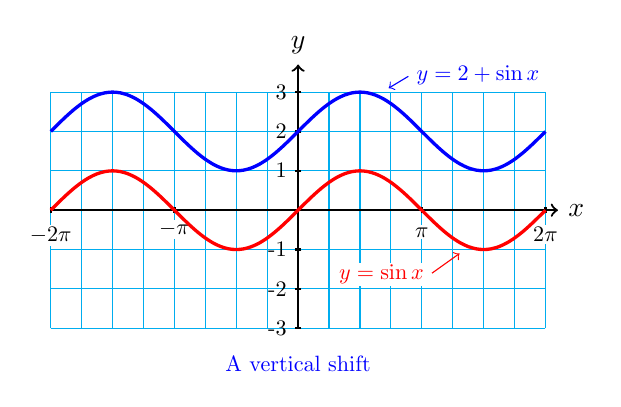
\begin{tikzpicture} [scale=1/2]
\draw[cyan] (-2*pi,-3) grid[xstep=pi/4, ystep=1] (2*pi,3);
\draw[black,thick,->](-2*pi,0)--(6.6,0) node[right]{$x$};
\draw[black,thick,->](0,-3)--(0,3.7) node[above]{$y$};
\foreach \y in {-3,-2,-1,1,2,3} \draw[black,thick] (0.08,\y)--++(-.16,0) node[left, scale=.8]{\y};
\draw[black,thick] (pi,.08)--++(0,-.16) node[below, yshift=-4, fill=white, inner sep=1, scale=.8] {$ \pi$};
\draw[black,thick] (2*pi,.08)--++(0,-.16) node[below, yshift=-4, fill=white, inner sep=1, scale=.8] {$ 2\pi$};
\draw[black,thick] (-pi,.08)--++(0,-.16) node[below, yshift=-2, fill=white, inner sep=1, scale=.8] {$ -\pi$};
\draw[black,thick] (-2*pi,.08)--++(0,-.16) node[below, yshift=-4, fill=white, inner sep=1, scale=.8] {$ -2\pi$};
\draw[samples=65, domain=-2*pi:2*pi, variable=\x, smooth,red, very thick] plot(\x,{sin(deg(\x))});
\draw[samples=65, domain=-2*pi:2*pi, variable=\x, smooth, blue, very thick] plot(\x,{2+sin(deg(\x))});
\draw[red, <-] (4.1,-1.1)--++(-.7,-.5) node[below left, xshift=-2, yshift=4, fill=white, inner sep=1, scale=.8] {$y=\sin x$};
\draw[blue, <-] (2.3,3.1)--++(.5,.3) node[above right, xshift=2, yshift=-4, fill=white, inner sep=1, scale=.8] {$y=2+\sin x$};
\node[text=blue, scale=.8] at (0,-3.9) {A vertical shift};
\end{tikzpicture}
\newline


fig-7-2-sinb scaling of sine

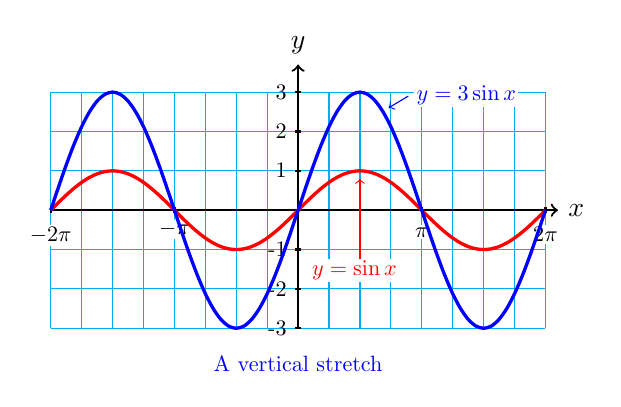
\begin{tikzpicture} [scale=1/2]
\draw[cyan] (-2*pi,-3) grid[xstep=pi/4, ystep=1] (2*pi,3);
\draw[black,thick,->](-2*pi,0)--(6.6,0) node[right]{$x$};
\draw[black,thick,->](0,-3)--(0,3.7) node[above]{$y$};
\foreach \y in {-3,-2,-1,1,2,3} \draw[black,thick] (0.08,\y)--++(-.16,0) node[left, scale=.8]{\y};
\draw[black,thick] (pi,.08)--++(0,-.16) node[below, yshift=-4, fill=white, inner sep=1, scale=.8] {$ \pi$};
\draw[black,thick] (2*pi,.08)--++(0,-.16) node[below, yshift=-4, fill=white, inner sep=1, scale=.8] {$ 2\pi$};
\draw[black,thick] (-pi,.08)--++(0,-.16) node[below, yshift=-2, fill=white, inner sep=1, scale=.8] {$ -\pi$};
\draw[black,thick] (-2*pi,.08)--++(0,-.16) node[below, yshift=-4, fill=white, inner sep=1, scale=.8] {$ -2\pi$};
\draw[samples=65, domain=-2*pi:2*pi, variable=\x, smooth,red, very thick] plot(\x,{sin(deg(\x))});
\draw[samples=65, domain=-2*pi:2*pi, variable=\x, smooth, blue, very thick] plot(\x,{3*sin(deg(\x))});
\draw[red, <-] (pi/2,0.8)--++(-0,-2.3) node[below , xshift=-2, yshift=4, fill=white, inner sep=1, scale=.8] {$y=\sin x$};
\draw[blue, <-] (2.3,2.6)--++(.5,.3) node[above right, xshift=2, yshift=-4, fill=white, inner sep=1, scale=.8] {$y=3\sin x$};
\node[text=blue, scale=.8] at (0,-3.9) {A vertical stretch};
\end{tikzpicture}
\newline


fig-7-2-sinc horizontal compression of sine

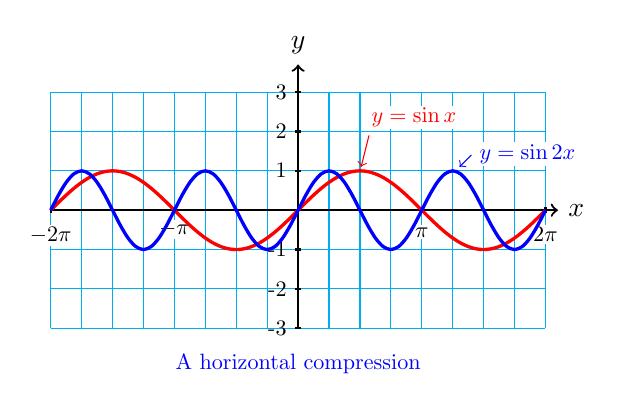
\begin{tikzpicture} [scale=1/2]
\draw[cyan] (-2*pi,-3) grid[xstep=pi/4, ystep=1] (2*pi,3);
\draw[black,thick,->](-2*pi,0)--(6.6,0) node[right]{$x$};
\draw[black,thick,->](0,-3)--(0,3.7) node[above]{$y$};
\foreach \y in {-3,-2,-1,1,2,3} \draw[black,thick] (0.08,\y)--++(-.16,0) node[left, scale=.8]{\y};
\draw[black,thick] (pi,.08)--++(0,-.16) node[below, yshift=-4, fill=white, inner sep=1, scale=.8] {$ \pi$};
\draw[black,thick] (2*pi,.08)--++(0,-.16) node[below, yshift=-4, fill=white, inner sep=1, scale=.8] {$ 2\pi$};
\draw[black,thick] (-pi,.08)--++(0,-.16) node[below, yshift=-2, fill=white, inner sep=1, scale=.8] {$ -\pi$};
\draw[black,thick] (-2*pi,.08)--++(0,-.16) node[below, yshift=-4, fill=white, inner sep=1, scale=.8] {$ -2\pi$};
\draw[samples=65, domain=-2*pi:2*pi, variable=\x, smooth,red, very thick] plot(\x,{sin(deg(\x))});
\draw[samples=65, domain=-2*pi:2*pi, variable=\x, smooth, blue, very thick] plot(\x,{sin(deg(2*\x))});
\draw[red, <-] (1.6,1.1)--++(0.2,.8) node[above right , yshift=-2, yshift=4, fill=white, inner sep=1, scale=.8] {$y=\sin x$};
\draw[blue, <-] (4.1,1.1)--++(.3,.3) node[above right, xshift=2, yshift=-4, fill=white, inner sep=1, scale=.8] {$y=\sin 2x$};
\node[text=blue, scale=.8] at (0,-3.9) {A horizontal compression};
\end{tikzpicture}
\newline


fig-7-2-sind horizontal shift of sine

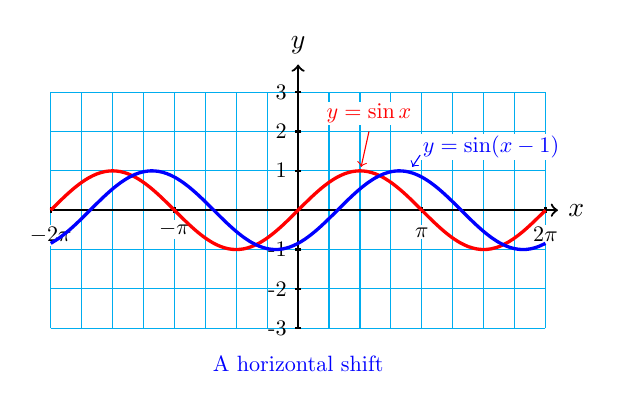
\begin{tikzpicture} [scale=1/2]
\draw[cyan] (-2*pi,-3) grid[xstep=pi/4, ystep=1] (2*pi,3);
\draw[black,thick,->](-2*pi,0)--(6.6,0) node[right]{$x$};
\draw[black,thick,->](0,-3)--(0,3.7) node[above]{$y$};
\foreach \y in {-3,-2,-1,1,2,3} \draw[black,thick] (0.08,\y)--++(-.16,0) node[left, scale=.8]{\y};
\draw[black,thick] (pi,.08)--++(0,-.16) node[below, yshift=-4, fill=white, inner sep=1, scale=.8] {$ \pi$};
\draw[black,thick] (2*pi,.08)--++(0,-.16) node[below, yshift=-4, fill=white, inner sep=1, scale=.8] {$ 2\pi$};
\draw[black,thick] (-pi,.08)--++(0,-.16) node[below, yshift=-2, fill=white, inner sep=1, scale=.8] {$ -\pi$};
\draw[black,thick] (-2*pi,.08)--++(0,-.16) node[below, yshift=-4, fill=white, inner sep=1, scale=.8] {$ -2\pi$};
\draw[samples=65, domain=-2*pi:2*pi, variable=\x, smooth,red, very thick] plot(\x,{sin(deg(\x))});
\draw[samples=65, domain=-2*pi:2*pi, variable=\x, smooth, blue, very thick] plot(\x,{sin(deg(\x-1))});
\draw[red, <-] (1.6,1.1)--++(0.2,.9) node[above  , yshift=-2, yshift=4, fill=white, inner sep=1, scale=.8] {$y=\sin x$};
\draw[blue, <-] (2.9,1.1)--++(.2,.3) node[above right, yshift=2, yshift=-4, fill=white, inner sep=1, scale=.8] {$y=\sin (x-1)$};
\node[text=blue, scale=.8] at (0,-3.9) {A horizontal shift};
\end{tikzpicture}
\newline


exam7-2-1 horizontal shift of sine

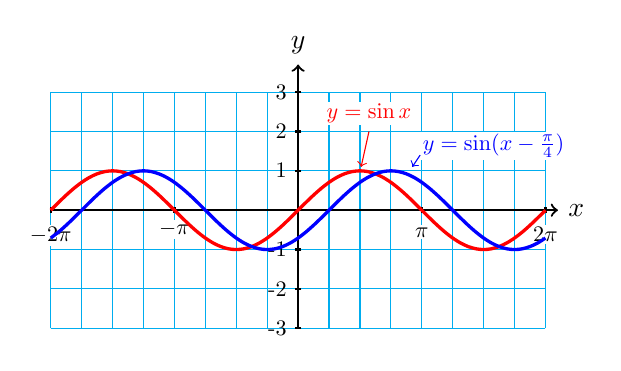
\begin{tikzpicture} [scale=1/2]
\draw[cyan] (-2*pi,-3) grid[xstep=pi/4, ystep=1] (2*pi,3);
\draw[black,thick,->](-2*pi,0)--(6.6,0) node[right]{$x$};
\draw[black,thick,->](0,-3)--(0,3.7) node[above]{$y$};
\foreach \y in {-3,-2,-1,1,2,3} \draw[black,thick] (0.08,\y)--++(-.16,0) node[left, scale=.8]{\y};
\draw[black,thick] (pi,.08)--++(0,-.16) node[below, yshift=-4, fill=white, inner sep=1, scale=.8] {$ \pi$};
\draw[black,thick] (2*pi,.08)--++(0,-.16) node[below, yshift=-4, fill=white, inner sep=1, scale=.8] {$ 2\pi$};
\draw[black,thick] (-pi,.08)--++(0,-.16) node[below, yshift=-2, fill=white, inner sep=1, scale=.8] {$ -\pi$};
\draw[black,thick] (-2*pi,.08)--++(0,-.16) node[below, yshift=-4, fill=white, inner sep=1, scale=.8] {$ -2\pi$};
\draw[samples=65, domain=-2*pi:2*pi, variable=\x, smooth,red, very thick] plot(\x,{sin(deg(\x))});
\draw[samples=65, domain=-2*pi:2*pi, variable=\x, smooth, blue, very thick] plot(\x,{sin(deg(\x-pi/4))});
\draw[red, <-] (1.6,1.1)--++(0.2,.9) node[above  , yshift=-2, yshift=4, fill=white, inner sep=1, scale=.8] {$y=\sin x$};
\draw[blue, <-] (2.9,1.1)--++(.2,.3) node[above right, yshift=2, yshift=-4, fill=white, inner sep=1, scale=.8] {$y=\sin (x-\frac{\pi}{4})$};
\end{tikzpicture}
\newline


exam7-2-2 transformation of sine

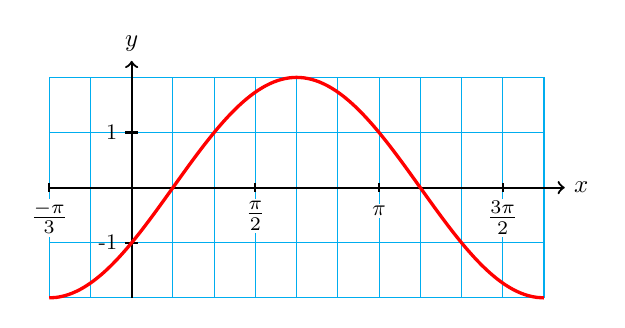
\begin{tikzpicture} [yscale=.7]
\draw[cyan] (-pi/3,-2) grid[xstep=pi/6, ystep=1] (5*pi/3,2);
\draw[black,thick,->](-pi/3,0)--(5.5,0) node[right, scale=.9]{$x$};
\draw[black,thick,->](0,-2)--(0,2.3) node[above, scale=.9]{$y$};
\foreach \y in {-1,1} \draw[black,thick] (0.08,\y)--++(-.16,0) node[left, scale=.8]{\y};
\draw[black,thick] (pi,.08)--++(0,-.16) node[below, yshift=-4, fill=white, inner sep=1, scale=.8] {$ \pi$};
\draw[black,thick] (-pi/3,.08)--++(0,-.16) node[below, yshift=-2, fill=white, inner sep=1] {$ \frac{-\pi}{3}$};
\draw[black,thick] (pi/2,.08)--++(0,-.16) node[below, yshift=-2, fill=white, inner sep=1] {$ \frac{\pi}{2}$};
\draw[black,thick] (3*pi/2,.08)--++(0,-.16) node[below, yshift=-2, fill=white, inner sep=1] {$ \frac{3\pi}{2}$};
\draw[samples=65, domain=-pi/3:5*pi/3, variable=\x, smooth,red, very thick] plot(\x,{-2*cos(deg(\x+pi/3))});
\end{tikzpicture}
\newline


exer7-2-2 grid

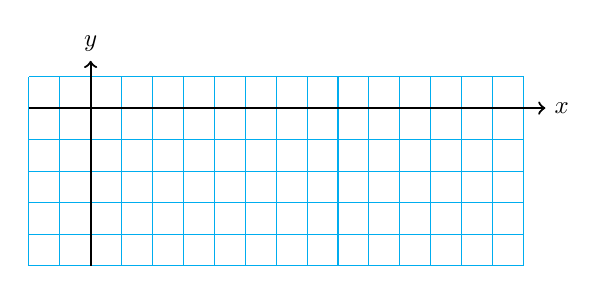
\begin{tikzpicture} [xscale=.75, yscale=.4]
\draw[cyan] (-pi/3,-5) grid[xstep=pi/6] (7*pi/3,1);
\draw[black,thick,->] (-pi/3,0)--(7.7,0) node[right, scale=.9]{$x$};
\draw[black,thick,->] (0,-5)--(0,1.5) node[above, scale=.9]{$y$};
\end{tikzpicture}
\newline


exer7-2-2ans -2+sin(x-pi/6)

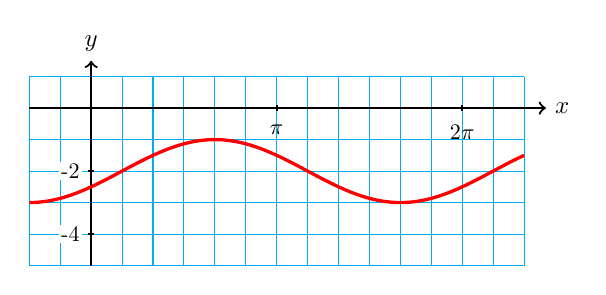
\begin{tikzpicture} [xscale=.75, yscale=.4]
\draw[cyan] (-pi/3,-5) grid[xstep=pi/6] (7*pi/3,1);
\draw[black,thick,->] (-pi/3,0)--(7.7,0) node[right, scale=.9]{$x$};
\draw[black,thick,->] (0,-5)--(0,1.5) node[above, scale=.9]{$y$};
\foreach \y in {-4,-2} \draw[black,thick] (.05,\y)--++(-.1,0) node[left, xshift=-2, fill=white, inner sep=1, scale=.8] {\y};
\draw[black,thick] (pi,.1)--++(0,-.2) node[below, yshift=-2, scale=.8] {$\pi$};
\draw[black,thick] (2*pi,.1)--++(0,-.2) node[below, yshift=-2, scale=.8] {$2\pi$};
\draw[samples=65, domain=-pi/3:7*pi/3, variable=\x, smooth,red, very thick] plot(\x,{-2+sin(deg(\x-pi/6))});
\end{tikzpicture}
\newline


fig-7-2-cta sin[2(x-pi/3)]

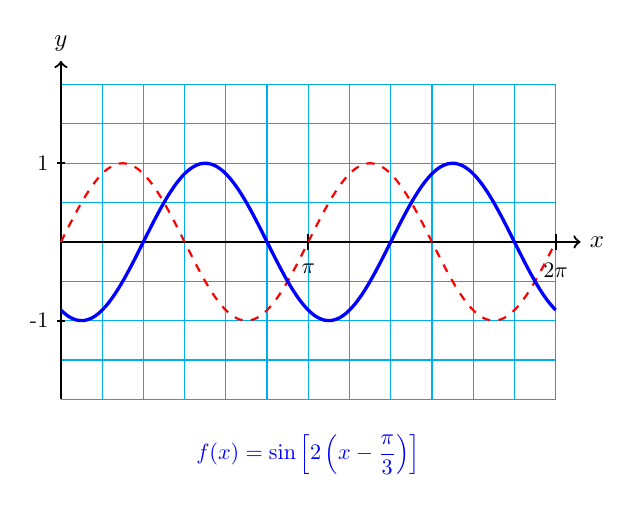
\begin{tikzpicture} [xscale=1, yscale=1]
\draw[cyan] (0,-2) grid[xstep=pi/6, ystep=1/2] (2*pi,2);
\draw[black,thick,->] (0,0)--(6.6,0) node[right, scale=.9]{$x$};
\draw[black,thick,->] (0,-2)--(0,2.3) node[above, scale=.9]{$y$};
\foreach \y in {-1,1} \draw[black,thick] (.05,\y)--++(-.1,0) node[left, xshift=-2, fill=white, inner sep=1, scale=.8] {\y};
\draw[black,thick] (pi,.1)--++(0,-.2) node[below, yshift=-2, scale=.8] {$\pi$};
\draw[black,thick] (2*pi,.1)--++(0,-.2) node[below, yshift=-2, scale=.8] {$2\pi$};
\draw[samples=65, domain=0:2*pi, variable=\x, smooth,red, thick, dashed] plot(\x,{ sin( (deg(2* \x) )});
\draw[samples=65, domain=0:2*pi, variable=\x, smooth,blue, very thick] plot(\x,{sin( (deg(2* (\x-pi/3)) )});
\node[text=blue, scale=.8] at (pi,-2.7) {$\displaystyle f(x)=\sin\left[2\left(x-\frac{\pi}{3}\right)\right]$};
\end{tikzpicture}
\newline


fig-7-2-ctb sin[2x-pi/3]

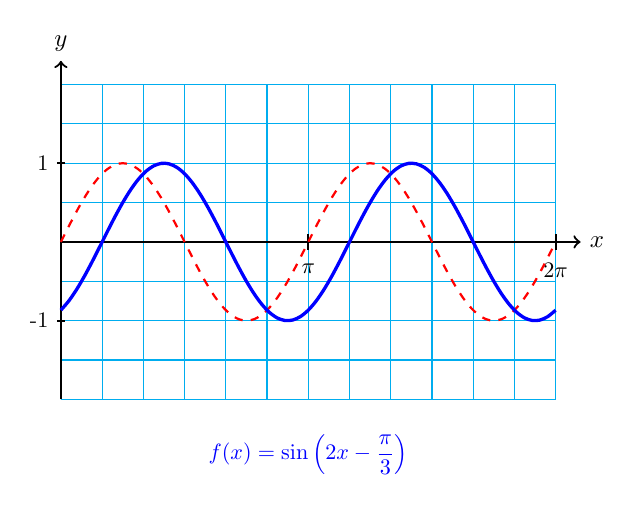
\begin{tikzpicture} [xscale=1, yscale=1]
\draw[cyan] (0,-2) grid[xstep=pi/6, ystep=1/2] (2*pi,2);
\draw[black,thick,->] (0,0)--(6.6,0) node[right, scale=.9]{$x$};
\draw[black,thick,->] (0,-2)--(0,2.3) node[above, scale=.9]{$y$};
\foreach \y in {-1,1} \draw[black,thick] (.05,\y)--++(-.1,0) node[left, xshift=-2, fill=white, inner sep=1, scale=.8] {\y};
\draw[black,thick] (pi,.1)--++(0,-.2) node[below, yshift=-2, scale=.8] {$\pi$};
\draw[black,thick] (2*pi,.1)--++(0,-.2) node[below, yshift=-2, scale=.8] {$2\pi$};
\draw[samples=65, domain=0:2*pi, variable=\x, smooth,red, thick, dashed] plot(\x,{ sin( (deg(2* \x) )});
\draw[samples=65, domain=0:2*pi, variable=\x, smooth,blue, very thick] plot(\x,{sin (deg( (2*\x-pi/3)) });
\node[text=blue, scale=.8] at (pi,-2.7) {$\displaystyle f(x)=\sin \left(2x-\frac{\pi}{3}\right)$};
\end{tikzpicture}
\newline


fig-7-2-ctc sin 2x

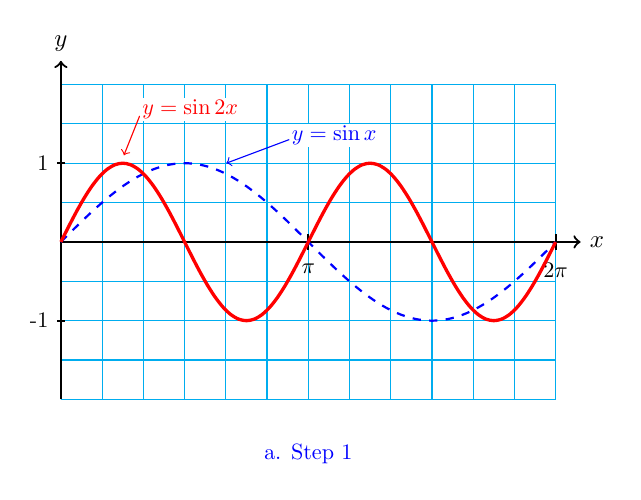
\begin{tikzpicture} [xscale=1, yscale=1]
\draw[cyan] (0,-2) grid[xstep=pi/6, ystep=1/2] (2*pi,2);
\draw[black,thick,->] (0,0)--(6.6,0) node[right, scale=.9]{$x$};
\draw[black,thick,->] (0,-2)--(0,2.3) node[above, scale=.9]{$y$};
\foreach \y in {-1,1} \draw[black,thick] (.05,\y)--++(-.1,0) node[left, xshift=-2, fill=white, inner sep=1, scale=.8] {\y};
\draw[black,thick] (pi,.1)--++(0,-.2) node[below, yshift=-2, scale=.8] {$\pi$};
\draw[black,thick] (2*pi,.1)--++(0,-.2) node[below, yshift=-2, scale=.8] {$2\pi$};
\draw[samples=65, domain=0:2*pi, variable=\x, smooth,blue, thick, dashed] plot(\x,{ sin( deg( \x) });
\draw[samples=65, domain=0:2*pi, variable=\x, smooth,red, very thick] plot(\x,{sin( deg(2* \x) });
\draw[blue, <-] (2.1,1.)--++(0.8,.3) node[above right, yshift=-3,  fill=white, inner sep=1, scale=.8] {$y=\sin x$};
\draw[red, <-] (0.8,1.1)--++(.2,.5) node[above right, yshift=-2, fill=white, inner sep=1, scale=.8] {$y=\sin 2x$};
\node[text=blue, scale=.8] at (pi,-2.7) {a. Step 1};
\end{tikzpicture}
\newline



fig-7-2-ctd sin 2(x-pi/3)

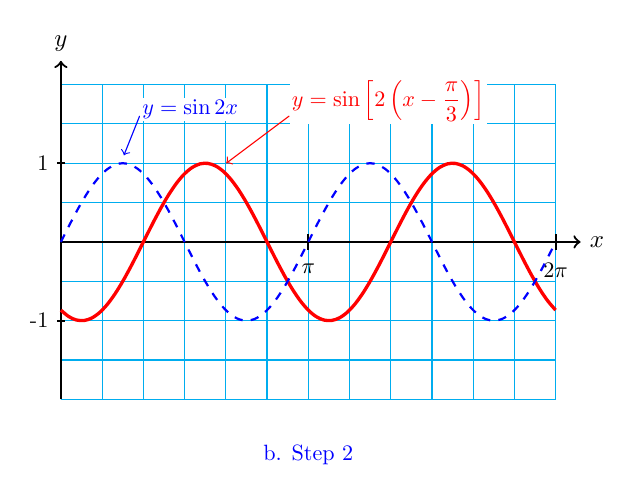
\begin{tikzpicture} [xscale=1, yscale=1]
\draw[cyan] (0,-2) grid[xstep=pi/6, ystep=1/2] (2*pi,2);
\draw[black,thick,->] (0,0)--(6.6,0) node[right, scale=.9]{$x$};
\draw[black,thick,->] (0,-2)--(0,2.3) node[above, scale=.9]{$y$};
\foreach \y in {-1,1} \draw[black,thick] (.05,\y)--++(-.1,0) node[left, xshift=-2, fill=white, inner sep=1, scale=.8] {\y};
\draw[black,thick] (pi,.1)--++(0,-.2) node[below, yshift=-2, scale=.8] {$\pi$};
\draw[black,thick] (2*pi,.1)--++(0,-.2) node[below, yshift=-2, scale=.8] {$2\pi$};
\draw[samples=65, domain=0:2*pi, variable=\x, smooth,red, very thick] plot(\x,{ sin( deg( 2*(\x- pi/3)) });
\draw[samples=65, domain=0:2*pi, variable=\x, smooth,blue, thick, dashed] plot(\x,{sin( deg(2* \x) });
\draw[red, <-] (2.1,1.)--++(0.8,.6) node[above right, yshift=-3,  fill=white, inner sep=1, scale=.8] {$\displaystyle y=\sin \left[ 2\left( x - \frac{\pi}{3}\right)\right]$};
\draw[blue, <-] (0.8,1.1)--++(.2,.5) node[above right, yshift=-2, fill=white, inner sep=1, scale=.8] {$y=\sin 2x$};
\node[text=blue, scale=.8] at (pi,-2.7) {b. Step 2};
\end{tikzpicture}
\newline


fig-7-2-cte sin (x - pi/3)

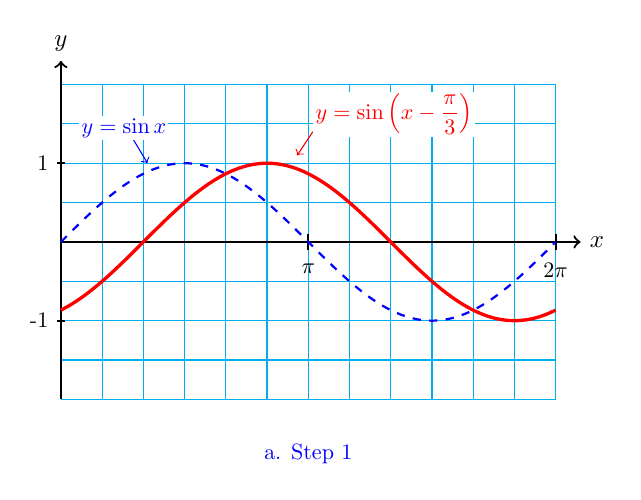
\begin{tikzpicture} [xscale=1, yscale=1]
\draw[cyan] (0,-2) grid[xstep=pi/6, ystep=1/2] (2*pi,2);
\draw[black,thick,->] (0,0)--(6.6,0) node[right, scale=.9]{$x$};
\draw[black,thick,->] (0,-2)--(0,2.3) node[above, scale=.9]{$y$};
\foreach \y in {-1,1} \draw[black,thick] (.05,\y)--++(-.1,0) node[left, xshift=-2, fill=white, inner sep=1, scale=.8] {\y};
\draw[black,thick] (pi,.1)--++(0,-.2) node[below, yshift=-2, scale=.8] {$\pi$};
\draw[black,thick] (2*pi,.1)--++(0,-.2) node[below, yshift=-2, scale=.8] {$2\pi$};
\draw[samples=65, domain=0:2*pi, variable=\x, smooth,blue, thick, dashed] plot(\x,{ sin( deg( \x) });
\draw[samples=65, domain=0:2*pi, variable=\x, smooth,red, very thick] plot(\x,{sin( deg( \x - pi/3 ) });
\draw[blue, <-] (1.1,1.)--++(-0.3,.5) node[above , yshift=-6,  fill=white, inner sep=1, scale=.8] {$y=\sin x$};
\draw[red, <-] (3.,1.1)--++(.2,.3) node[above right, yshift=-2, fill=white, inner sep=1, scale=.8] {$\displaystyle y=\sin \left(x- \frac{\pi}{3}\right)$};
\node[text=blue, scale=.8] at (pi,-2.7) {a. Step 1};
\end{tikzpicture}
\newline



fig-7-2-ctd sin 2(x-pi/3)

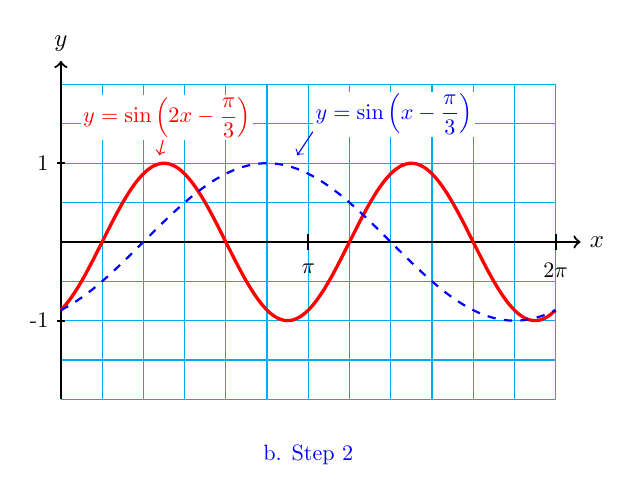
\begin{tikzpicture} [xscale=1, yscale=1]
\draw[cyan] (0,-2) grid[xstep=pi/6, ystep=1/2] (2*pi,2);
\draw[black,thick,->] (0,0)--(6.6,0) node[right, scale=.9]{$x$};
\draw[black,thick,->] (0,-2)--(0,2.3) node[above, scale=.9]{$y$};
\foreach \y in {-1,1} \draw[black,thick] (.05,\y)--++(-.1,0) node[left, xshift=-2, fill=white, inner sep=1, scale=.8] {\y};
\draw[black,thick] (pi,.1)--++(0,-.2) node[below, yshift=-2, scale=.8] {$\pi$};
\draw[black,thick] (2*pi,.1)--++(0,-.2) node[below, yshift=-2, scale=.8] {$2\pi$};
\draw[samples=65, domain=0:2*pi, variable=\x, smooth,red, very thick] plot(\x,{ sin(  deg( 2*\x - pi/3  });
\draw[samples=65, domain=0:2*pi, variable=\x, smooth,blue, dashed, thick] plot(\x,{sin( deg( \x - pi/3 ) });
\draw[red, <-] (1.25,1.1)--++(0.1,.4) node[above , yshift=-6,  fill=white, inner sep=1, scale=.8] {$\displaystyle y=\sin \left(2x - \frac{\pi}{3}\right)$};
\draw[blue, <-] (3.,1.1)--++(.2,.3) node[above right, yshift=-2, fill=white, inner sep=1, scale=.8] {$\displaystyle y=\sin \left(x- \frac{\pi}{3}\right)$};
\node[text=blue, scale=.8] at (pi,-2.7) {b. Step 2};
\end{tikzpicture}
\newline



exam7-2-3 4cos3(x+pi/3)-2

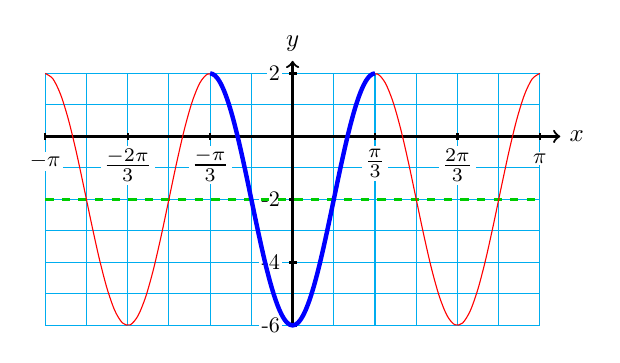
\begin{tikzpicture} [xscale=1, yscale=.4]
\draw[cyan] (-pi,-6) grid[xstep=pi/6] (pi,2);
\draw[black,thick,->] (-pi,0)--(3.4,0) node[right, scale=.9]{$x$};
\draw[black,thick,->] (0,-6)--(0,2.4) node[above, scale=.9]{$y$};
\foreach \y in {-6,-4,-2,2} \draw[black,thick] (.05,\y)--++(-.1,0) node[left, xshift=-2, fill=white, inner sep=1, scale=.8] {\y};
\draw[black,thick] (-pi,.1)--++(0,-.2) node[below, yshift=-4, fill=white, inner sep=1, scale=.8] {$-\pi$};
\draw[black,thick] (pi,.1)--++(0,-.2) node[below, yshift=-4, fill=white, inner sep=1, scale=.8] {$\pi$};
\draw[black,thick] (-2*pi/3,.1)--++(0,-.2) node[below, yshift=-2, fill=white, inner sep=1] {$\frac{-2\pi}{3}$};
\draw[black,thick] (-pi/3,.1)--++(0,-.2) node[below, yshift=-2, fill=white, inner sep=1] {$\frac{-\pi}{3}$};
\draw[black,thick] (2*pi/3,.1)--++(0,-.2) node[below, yshift=-2, fill=white, inner sep=1] {$\frac{2\pi}{3}$};
\draw[black,thick] (pi/3,.1)--++(0,-.2) node[below, yshift=-2, fill=white, inner sep=1] {$\frac{\pi}{3}$};
\draw[green!80!black, very thick, dashed] (-pi,-2)--(pi,-2);
\draw[samples=65, domain=-pi:pi, variable=\x, smooth,red] plot(\x,{ 4*cos( 3* deg( \x + pi/3))-2 });
\draw[samples=65, domain=-pi/3:pi/3, variable=\x, smooth,blue, ultra thick] plot(\x,{ 4*cos( 3* deg( \x + pi/3))-2 });
\end{tikzpicture}
\newline


exer7-2-3ans 150-25 cos(4x-pi/2)

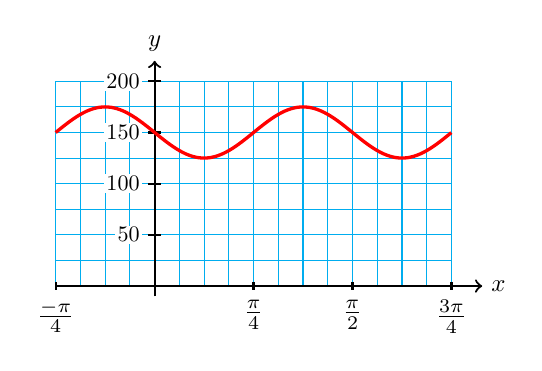
\begin{tikzpicture} [xscale=1.6, yscale=.013]
\draw[cyan] (-pi/4,0) grid[xstep=pi/16, ystep=25] (3*pi/4,200);
\draw[black,thick,->] (-pi/4,0)--(2.6,0) node[right, scale=.9]{$x$};
\draw[black,thick,->] (0,-10)--(0,220) node[above, scale=.9]{$y$};
\foreach \y in {50,100, 150,200} \draw[black,thick] (.05,\y)--++(-.1,0) node[left, xshift=-2, fill=white, inner sep=1, scale=.8] {\y};
\draw[black,thick] (pi/4,4)--++(0,-8) node[below] {$\frac{\pi}{4}$};
\draw[black,thick] (-pi/4,4)--++(0,-8) node[below] {$\frac{-\pi}{4}$};
\draw[black,thick] (pi/2,4)--++(0,-8) node[below] {$\frac{\pi}{2}$};
\draw[black,thick] (3*pi/4,4)--++(0,-8) node[below] {$\frac{3\pi}{4}$};
\draw[samples=65, domain=-pi/4:3*pi/4, variable=\x, smooth,red, very thick] plot(\x,{150-25*cos( deg(4*\x-pi/2))});
\end{tikzpicture}
\newline


exam7-2-4 4 cos(x-pi/6)

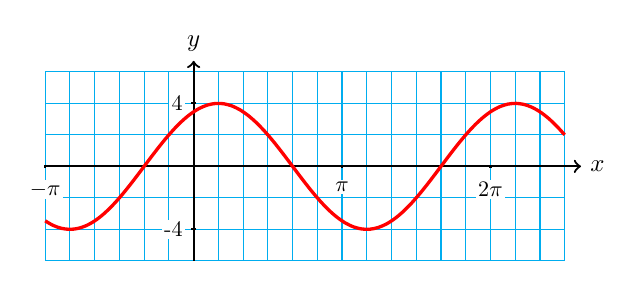
\begin{tikzpicture} [xscale=.6, yscale=.2]
\draw[cyan] (-pi,-6) grid[xstep=pi/6, ystep=2] (5*pi/2,6);
\draw[black,thick,->] (-pi,0)--(8.2,0) node[right, scale=.9]{$x$};
\draw[black,thick,->] (0,-6)--(0,6.7) node[above, scale=.9]{$y$};
\foreach \y in {-4,4} \draw[black,thick] (.05,\y)--++(-.1,0) node[left, xshift=-2, fill=white, inner sep=1, scale=.8] {\y};
\draw[black,thick] (-pi,0.1)--++(0,-.2) node[below, yshift=-4, fill=white, inner sep=1, scale=.8] {$-\pi$};
\draw[black,thick] (pi,0.1)--++(0,-.2) node[below, yshift=-4, fill=white, inner sep=1, scale=.8] {$\pi$};
\draw[black,thick] (2*pi,0.1)--++(0,-.2) node[below, yshift=-4, fill=white, inner sep=1, scale=.8] {$2\pi$};
\draw[samples=65, domain=-pi:5*pi/2, variable=\x, smooth,red, very thick] plot(\x,{4*cos( deg(\x-pi/6))});
\end{tikzpicture}
\newline


exer7-2-4 4 6 sin( x - pi/4)

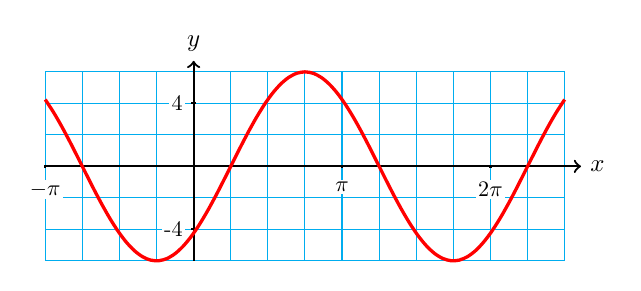
\begin{tikzpicture} [xscale=.6, yscale=.2]
\draw[cyan] (-pi,-6) grid[xstep=pi/4, ystep=2] (5*pi/2,6);
\draw[black,thick,->] (-pi,0)--(8.2,0) node[right, scale=.9]{$x$};
\draw[black,thick,->] (0,-6)--(0,6.7) node[above, scale=.9]{$y$};
\foreach \y in {-4,4} \draw[black,thick] (.05,\y)--++(-.1,0) node[left, xshift=-2, fill=white, inner sep=1, scale=.8] {\y};
\draw[black,thick] (-pi,0.1)--++(0,-.2) node[below, yshift=-4, fill=white, inner sep=1, scale=.8] {$-\pi$};
\draw[black,thick] (pi,0.1)--++(0,-.2) node[below, yshift=-4, fill=white, inner sep=1, scale=.8] {$\pi$};
\draw[black,thick] (2*pi,0.1)--++(0,-.2) node[below, yshift=-4, fill=white, inner sep=1, scale=.8] {$2\pi$};
\draw[samples=65, domain=-pi:5*pi/2, variable=\x, smooth,red, very thick] plot(\x,{6*sin( deg(\x-pi/4))});
\end{tikzpicture}
\newline


ar7-2-1ans parabolas

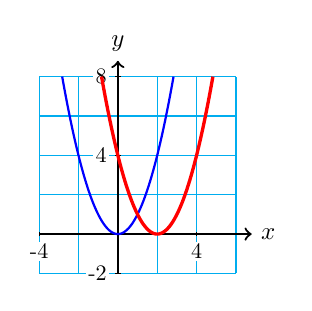
\begin{tikzpicture} [scale=.25]
\draw[cyan] (-4,-2) grid[step=2] (6,8);
\draw[black,thick,->] (-4,0)--(6.8,0) node[right, scale=.9]{$x$};
\draw[black,thick,->] (0,-2)--(0,8.8) node[above, scale=.9]{$y$};
\foreach \x in {-4,4} \draw[black] (\x,.1)--++(0,-.2) node[below, yshift=-2, fill=white, inner sep=1, scale=.8] {\x};
\foreach \y in {-2,4,8} \draw[black] (.15,\y)--++(-.3,0) node[left, xshift=-2, fill=white, inner sep=1, scale=.8] {\y};
\draw[samples=65, domain={-2*sqrt(2)}:{2*sqrt(2)}, variable=\x, smooth,blue, thick] plot(\x,{ (\x)^2 });
\draw[samples=65, domain={2-2*sqrt(2)}:{2+2*sqrt(2)}, variable=\x, smooth,red, very thick] plot(\x,{ (\x-2)^2 });
\end{tikzpicture}
\newline


ar7-2-2ans square roots

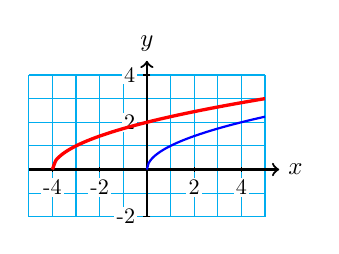
\begin{tikzpicture} [scale=.3]
\draw[cyan] (-5,-2) grid (5,4);
\draw[black,thick,->] (-5,0)--(5.6,0) node[right, scale=.9]{$x$};
\draw[black,thick,->] (0,-2)--(0,4.6) node[above, scale=.9]{$y$};
\foreach \x in {-4,4, -2,2} \draw[black] (\x,.1)--++(0,-.2) node[below, yshift=-2, fill=white, inner sep=1, scale=.8] {\x};
\foreach \y in {-2,2,4} \draw[black] (.15,\y)--++(-.3,0) node[left, xshift=-2, fill=white, inner sep=1, scale=.8] {\y};
\draw[samples=65, domain=0:5, variable=\x, smooth,blue, thick] plot(\x,{ sqrt(\x) });
\draw[samples=65, domain=-4:5, variable=\x, smooth,red, very thick] plot(\x,{ sqrt(\x+4) });
\end{tikzpicture}
\newline


ar7-2-3ans reciprocals

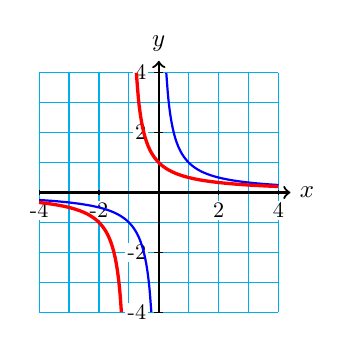
\begin{tikzpicture} [scale=.38]
\draw[cyan] (-4,-4) grid (4,4);
\draw[black,thick,->] (-4,0)--(4.4,0) node[right, scale=.9]{$x$};
\draw[black,thick,->] (0,-4)--(0,4.4) node[above, scale=.9]{$y$};
\foreach \x in {-4,4, -2,2} \draw[black] (\x,.1)--++(0,-.2) node[below, yshift=-2, fill=white, inner sep=1, scale=.8] {\x};
\foreach \y in {-2,2,4,-4} \draw[black] (.15,\y)--++(-.3,0) node[left, xshift=-2, fill=white, inner sep=1, scale=.8] {\y};
\draw[samples=65, domain=-4:-1/4, variable=\x, smooth,blue, thick] plot(\x,{ 1/(\x) });
\draw[samples=65, domain=1/4:4, variable=\x, smooth,blue, thick] plot(\x,{ 1/(\x) });
\draw[samples=65, domain=-4:-1/4-1, variable=\x, smooth,red, very thick] plot(\x,{ 1/(\x+1) });
\draw[samples=65, domain=1/4-1:4, variable=\x, smooth,red, very thick] plot(\x,{ 1/(\x+1) });
\end{tikzpicture}
\newline
\newline


ar7-2-4ans inverse squares

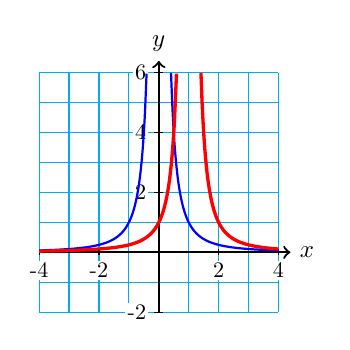
\begin{tikzpicture} [scale=.38]
\draw[cyan] (-4,-2) grid (4,6);
\draw[black,thick,->] (-4,0)--(4.4,0) node[right, scale=.9]{$x$};
\draw[black,thick,->] (0,-2)--(0,6.4) node[above, scale=.9]{$y$};
\foreach \x in {-4,4, -2,2} \draw[black] (\x,.1)--++(0,-.2) node[below, yshift=-2, fill=white, inner sep=1, scale=.8] {\x};
\foreach \y in {-2,2,4,6} \draw[black] (.15,\y)--++(-.3,0) node[left, xshift=-2, fill=white, inner sep=1, scale=.8] {\y};
\draw[samples=65, domain=-4:-1/sqrt(6), variable=\x, smooth,blue, thick] plot(\x,{ 1/(\x)^2 });
\draw[samples=65, domain=1/sqrt(6):4, variable=\x, smooth,blue, thick] plot(\x,{  1/(\x)^2 });
\draw[samples=65, domain=-4:-1/1/sqrt(6)+1, variable=\x, smooth,red, very thick] plot(\x,{  1/(\x -1)^2 });
\draw[samples=65, domain=1/1/sqrt(6)+1:4, variable=\x, smooth,red, very thick] plot(\x,{  1/(\x -1)^2 });
\end{tikzpicture}
\newline



ar7-2-5ans absolute values

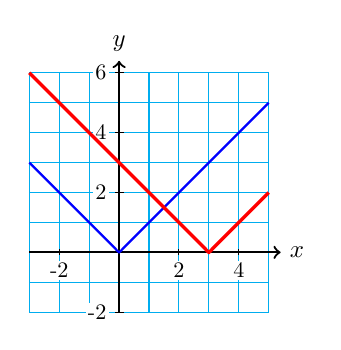
\begin{tikzpicture} [scale=.38]
\draw[cyan] (-3,-2) grid (5,6);
\draw[black,thick,->] (-3,0)--(5.4,0) node[right, scale=.9]{$x$};
\draw[black,thick,->] (0,-2)--(0,6.4) node[above, scale=.9]{$y$};
\foreach \x in {4, -2,2} \draw[black] (\x,.1)--++(0,-.2) node[below, yshift=-2, fill=white, inner sep=1, scale=.8] {\x};
\foreach \y in {-2,2,4,6} \draw[black] (.15,\y)--++(-.3,0) node[left, xshift=-2, fill=white, inner sep=1, scale=.8] {\y};
\draw[samples=65, domain=-3:5, variable=\x, smooth,blue, thick] plot(\x,{  abs(\x)});
\draw[samples=65, domain=-3:5, variable=\x, smooth,red, very thick] plot(\x,{ abs(\x-3 });
\end{tikzpicture}
\newline



ar7-2-6ans absolute values

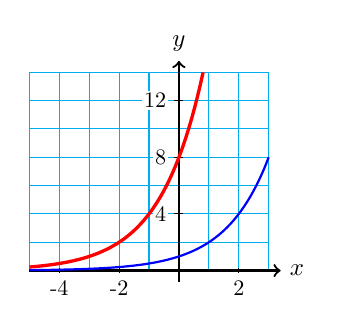
\begin{tikzpicture} [xscale=.38, yscale=.18]
\draw[cyan] (-5,0) grid[ystep=2] (3,14);
\draw[black,thick,->] (-5,0)--(3.4,0) node[right, scale=.9]{$x$};
\draw[black,thick,->] (0,-.8)--(0,14.8) node[above, scale=.9]{$y$};
\foreach \x in {-4,-2,2} \draw[black] (\x,.2)--++(0,-.4) node[below, yshift=-2, fill=white, inner sep=1, scale=.8] {\x};
\foreach \y in {4,8,12} \draw[black] (.15,\y)--++(-.3,0) node[left, xshift=-2, fill=white, inner sep=1, scale=.8] {\y};
\draw[samples=65, domain=-5:3, variable=\x, smooth,blue, thick] plot(\x,{  2^(\x)});
\draw[samples=65, domain=-5:{log2(14)-3}, variable=\x, smooth,red, very thick] plot(\x,{ 2^(\x+3 });
\end{tikzpicture}
\newline


hp7-2-1 grid

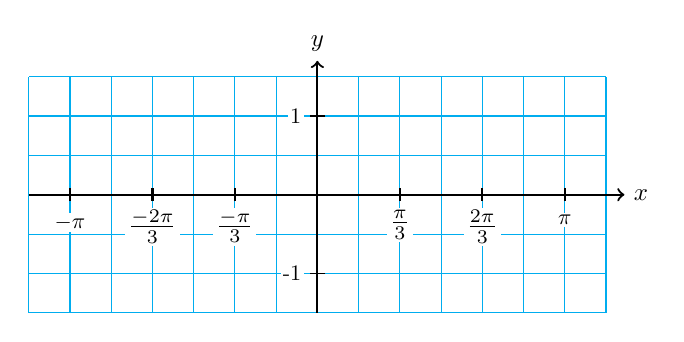
\begin{tikzpicture}
\draw[cyan] (-7*pi/6,-3/2) grid[xstep=pi/6, ystep=1/2] (7*pi/6,3/2);
\draw[black,thick,->] (-7*pi/6,0)--(3.9,0) node[right, scale=.9]{$x$};
\draw[black,thick,->] (0,-1.5)--(0,1.7) node[above, scale=.9]{$y$};
\foreach \y in {-1,1} \draw(.1,\y)--++(-.2,0) node[left, xshift=-2, fill=white, inner sep=1, scale=.8] {\y};
\draw[black,thick] (-pi,.08)--++(0,-.16) node[below, yshift=-4, fill=white, inner sep=1, scale=.8] {$-\pi$};
\draw[black,thick] (pi,.08)--++(0,-.16) node[below, yshift=-4, fill=white, inner sep=1, scale=.8] {$\pi$};
\draw[black,thick] (-2*pi/3,.08)--++(0,-.16) node[below, yshift=-2, fill=white, inner sep=1] {$\frac{-2\pi}{3}$};
\draw[black,thick] (-pi/3,.08)--++(0,-.16) node[below, yshift=-2, fill=white, inner sep=1] {$\frac{-\pi}{3}$};
\draw[black,thick] (pi/3,.08)--++(0,-.16) node[below, yshift=-2, fill=white, inner sep=1] {$\frac{\pi}{3}$};
\draw[black,thick] (2*pi/3,.08)--++(0,-.16) node[below, yshift=-2, fill=white, inner sep=1] {$\frac{2\pi}{3}$};
\end{tikzpicture}
\newline


hp7-2-1ans grid

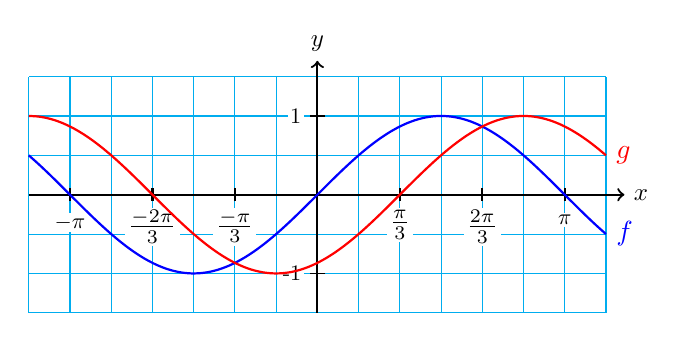
\begin{tikzpicture}
\draw[cyan] (-7*pi/6,-3/2) grid[xstep=pi/6, ystep=1/2] (7*pi/6,3/2);
\draw[black,thick,->] (-7*pi/6,0)--(3.9,0) node[right, scale=.9]{$x$};
\draw[black,thick,->] (0,-1.5)--(0,1.7) node[above, scale=.9]{$y$};
\foreach \y in {-1,1} \draw(.1,\y)--++(-.2,0) node[left, xshift=-2, fill=white, inner sep=1, scale=.8] {\y};
\draw[black,thick] (-pi,.08)--++(0,-.16) node[below, yshift=-4, fill=white, inner sep=1, scale=.8] {$-\pi$};
\draw[black,thick] (pi,.08)--++(0,-.16) node[below, yshift=-4, fill=white, inner sep=1, scale=.8] {$\pi$};
\draw[black,thick] (-2*pi/3,.08)--++(0,-.16) node[below, yshift=-2, fill=white, inner sep=1] {$\frac{-2\pi}{3}$};
\draw[black,thick] (-pi/3,.08)--++(0,-.16) node[below, yshift=-2, fill=white, inner sep=1] {$\frac{-\pi}{3}$};
\draw[black,thick] (pi/3,.08)--++(0,-.16) node[below, yshift=-2, fill=white, inner sep=1] {$\frac{\pi}{3}$};
\draw[black,thick] (2*pi/3,.08)--++(0,-.16) node[below, yshift=-2, fill=white, inner sep=1] {$\frac{2\pi}{3}$};
\draw[samples=65,domain={-7*pi/6}:{7*pi/6}, smooth, blue, thick] plot(\x, {sin(deg(\x)}) node[right] {$f$};
\draw[samples=65,domain={-7*pi/6}:{7*pi/6}, smooth, red, thick] plot(\x, {sin(deg(\x - pi/3)}) node[right] {$g$};
\end{tikzpicture}
\newline


hp7-2-3 grid

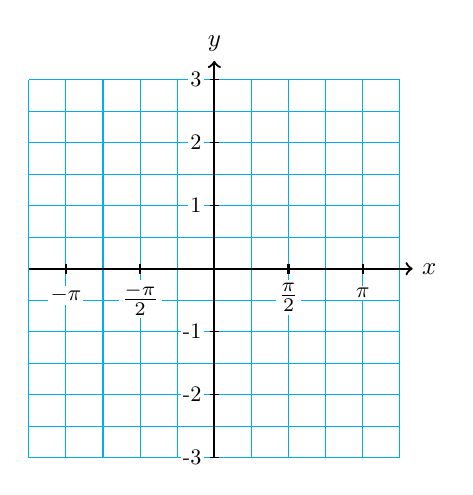
\begin{tikzpicture} [xscale=.6, yscale=.8]
\draw[cyan] (-5*pi/4,-3) grid[xstep=pi/4, ystep=1/2] (5*pi/4,3);
\draw[black,thick,->] (-5*pi/4,0)--(4.2,0) node[right, scale=.9]{$x$};
\draw[black,thick,->] (0,-3)--(0,3.3) node[above, scale=.9]{$y$};
\foreach \y in {-1,1,-2,2,-3,3} \draw(.1,\y)--++(-.2,0) node[left, xshift=-2, fill=white, inner sep=1, scale=.8] {\y};
\draw[black,thick] (-pi,.08)--++(0,-.16) node[below, yshift=-4, fill=white, inner sep=1, scale=.8] {$-\pi$};
\draw[black,thick] (pi,.08)--++(0,-.16) node[below, yshift=-4, fill=white, inner sep=1, scale=.8] {$\pi$};
\draw[black,thick] (-pi/2,.08)--++(0,-.16) node[below, yshift=-2, fill=white, inner sep=1] {$\frac{-\pi}{2}$};
\draw[black,thick] (pi/2,.08)--++(0,-.16) node[below, yshift=-2, fill=white, inner sep=1] {$\frac{\pi}{2}$};
\end{tikzpicture}
\newline


hp7-2-3ans translated tan

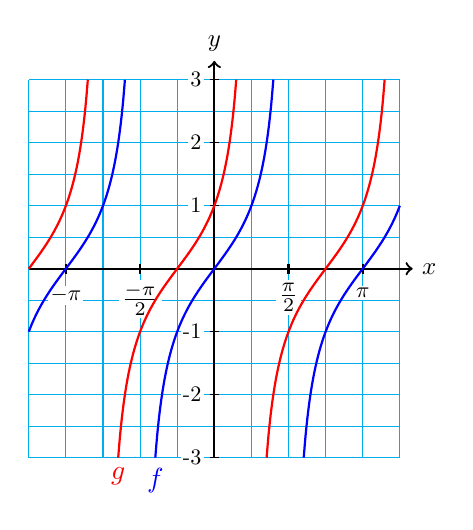
\begin{tikzpicture} [xscale=.6, yscale=.8]
\draw[cyan] (-5*pi/4,-3) grid[xstep=pi/4, ystep=1/2] (5*pi/4,3);
\draw[black,thick,->] (-5*pi/4,0)--(4.2,0) node[right, scale=.9]{$x$};
\draw[black,thick,->] (0,-3)--(0,3.3) node[above, scale=.9]{$y$};
\foreach \y in {-1,1,-2,2,-3,3} \draw(.1,\y)--++(-.2,0) node[left, xshift=-2, fill=white, inner sep=1, scale=.8] {\y};
\draw[black,thick] (-pi,.08)--++(0,-.16) node[below, yshift=-4, fill=white, inner sep=1, scale=.8] {$-\pi$};
\draw[black,thick] (pi,.08)--++(0,-.16) node[below, yshift=-4, fill=white, inner sep=1, scale=.8] {$\pi$};
\draw[black,thick] (-pi/2,.08)--++(0,-.16) node[below, yshift=-2, fill=white, inner sep=1] {$\frac{-\pi}{2}$};
\draw[black,thick] (pi/2,.08)--++(0,-.16) node[below, yshift=-2, fill=white, inner sep=1] {$\frac{\pi}{2}$};
\draw[samples=65,domain={atan(3)*pi/180}:{-atan(3)*pi/180}, smooth, blue, thick] plot(\x, {tan(deg(\x)}) node[below] {$f$};
\draw[samples=65,domain={-5*pi/4}:{atan(3)*pi/180-pi}, smooth, blue, thick] plot(\x, {tan(deg(\x)}) ;
\draw[samples=65,domain={5*pi/4}:{-atan(3)*pi/180+pi}, smooth, blue, thick] plot(\x, {tan(deg(\x)}) ;
\draw[samples=65,domain={atan(3)*pi/180}:{-atan(3)*pi/180}, smooth, red, thick] plot(\x-pi/4, {tan(deg(\x )}) node[below] {$g$};
\draw[samples=65,domain={-5*pi/4}:{atan(3)*pi/180-pi-pi/4}, smooth, red, thick] plot(\x, {tan(deg(\x+pi/4)}) ;
\draw[samples=65,domain={-atan(3)*pi/180+pi-pi/4}:{atan(3)*pi/180+3*pi/4}, smooth, red, thick] plot(\x, {tan(deg(\x+pi/4)}) ;
\end{tikzpicture}
\newline


hp7-2-5 grid

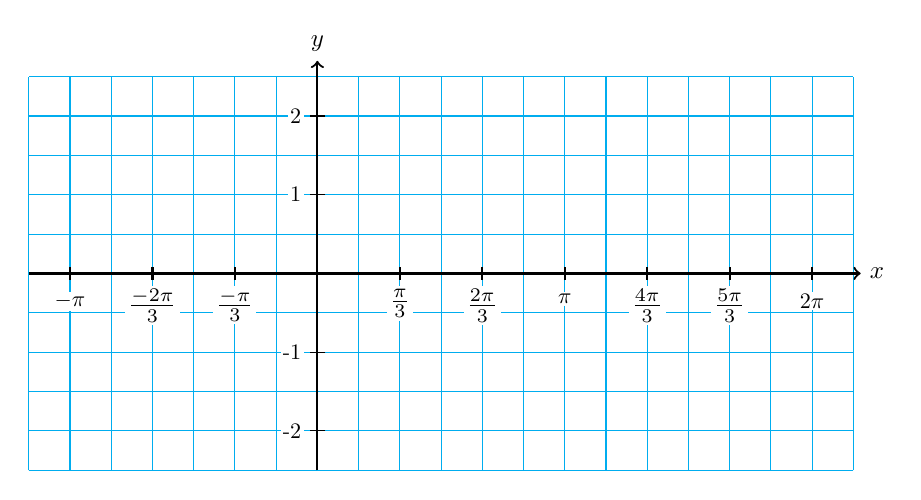
\begin{tikzpicture}
\draw[cyan] (-7*pi/6,-5/2) grid[xstep=pi/6, ystep=1/2] (13*pi/6,5/2);
\draw[black,thick,->] (-7*pi/6,0)--(6.9,0) node[right, scale=.9]{$x$};
\draw[black,thick,->] (0,-2.5)--(0,2.7) node[above, scale=.9]{$y$};
\foreach \y in {-1,1,-2,2} \draw(.1,\y)--++(-.2,0) node[left, xshift=-2, fill=white, inner sep=1, scale=.8] {\y};
\draw[black,thick] (-pi,.08)--++(0,-.16) node[below, yshift=-4, fill=white, inner sep=1, scale=.8] {$-\pi$};
\draw[black,thick] (pi,.08)--++(0,-.16) node[below, yshift=-4, fill=white, inner sep=1, scale=.8] {$\pi$};
\draw[black,thick] (-2*pi/3,.08)--++(0,-.16) node[below, yshift=-2, fill=white, inner sep=1] {$\frac{-2\pi}{3}$};
\draw[black,thick] (-pi/3,.08)--++(0,-.16) node[below, yshift=-2, fill=white, inner sep=1] {$\frac{-\pi}{3}$};
\draw[black,thick] (pi/3,.08)--++(0,-.16) node[below, yshift=-2, fill=white, inner sep=1] {$\frac{\pi}{3}$};
\draw[black,thick] (2*pi/3,.08)--++(0,-.16) node[below, yshift=-2, fill=white, inner sep=1] {$\frac{2\pi}{3}$};
\draw[black,thick] (4*pi/3,.08)--++(0,-.16) node[below, yshift=-2, fill=white, inner sep=1] {$\frac{4\pi}{3}$};
\draw[black,thick] (5*pi/3,.08)--++(0,-.16) node[below, yshift=-2, fill=white, inner sep=1] {$\frac{5\pi}{3}$};
\draw[black,thick] (2*pi/3,.08)--++(0,-.16) node[below, yshift=-2, fill=white, inner sep=1] {$\frac{2\pi}{3}$};
\draw[black,thick] (2*pi,.08)--++(0,-.16) node[below, yshift=-4, fill=white, inner sep=1, scale=.8] {$2\pi$};
\end{tikzpicture}
\newline


hp7-2-5ans -2 cos(x + pi/6)

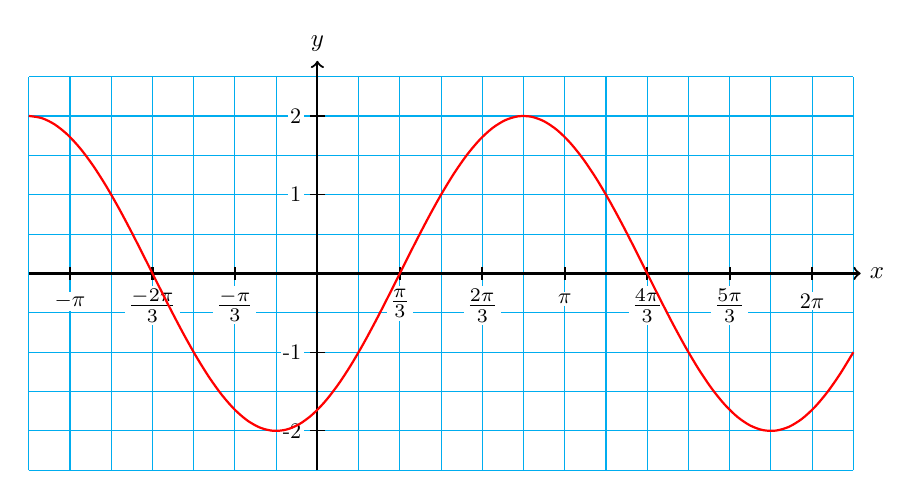
\begin{tikzpicture}
\draw[cyan] (-7*pi/6,-5/2) grid[xstep=pi/6, ystep=1/2] (13*pi/6,5/2);
\draw[black,thick,->] (-7*pi/6,0)--(6.9,0) node[right, scale=.9]{$x$};
\draw[black,thick,->] (0,-2.5)--(0,2.7) node[above, scale=.9]{$y$};
\foreach \y in {-1,1,-2,2} \draw(.1,\y)--++(-.2,0) node[left, xshift=-2, fill=white, inner sep=1, scale=.8] {\y};
\draw[black,thick] (-pi,.08)--++(0,-.16) node[below, yshift=-4, fill=white, inner sep=1, scale=.8] {$-\pi$};
\draw[black,thick] (pi,.08)--++(0,-.16) node[below, yshift=-4, fill=white, inner sep=1, scale=.8] {$\pi$};
\draw[black,thick] (-2*pi/3,.08)--++(0,-.16) node[below, yshift=-2, fill=white, inner sep=1] {$\frac{-2\pi}{3}$};
\draw[black,thick] (-pi/3,.08)--++(0,-.16) node[below, yshift=-2, fill=white, inner sep=1] {$\frac{-\pi}{3}$};
\draw[black,thick] (pi/3,.08)--++(0,-.16) node[below, yshift=-2, fill=white, inner sep=1] {$\frac{\pi}{3}$};
\draw[black,thick] (2*pi/3,.08)--++(0,-.16) node[below, yshift=-2, fill=white, inner sep=1] {$\frac{2\pi}{3}$};
\draw[black,thick] (4*pi/3,.08)--++(0,-.16) node[below, yshift=-2, fill=white, inner sep=1] {$\frac{4\pi}{3}$};
\draw[black,thick] (5*pi/3,.08)--++(0,-.16) node[below, yshift=-2, fill=white, inner sep=1] {$\frac{5\pi}{3}$};
\draw[black,thick] (2*pi/3,.08)--++(0,-.16) node[below, yshift=-2, fill=white, inner sep=1] {$\frac{2\pi}{3}$};
\draw[black,thick] (2*pi,.08)--++(0,-.16) node[below, yshift=-4, fill=white, inner sep=1, scale=.8] {$2\pi$};
\draw[samples=65,domain={-7*pi/6}:{13*pi/6}, smooth, red, thick] plot(\x, {-2*cos(deg(\x+pi/6)}) ;
\end{tikzpicture}
\newline


hp7-2-6 grid

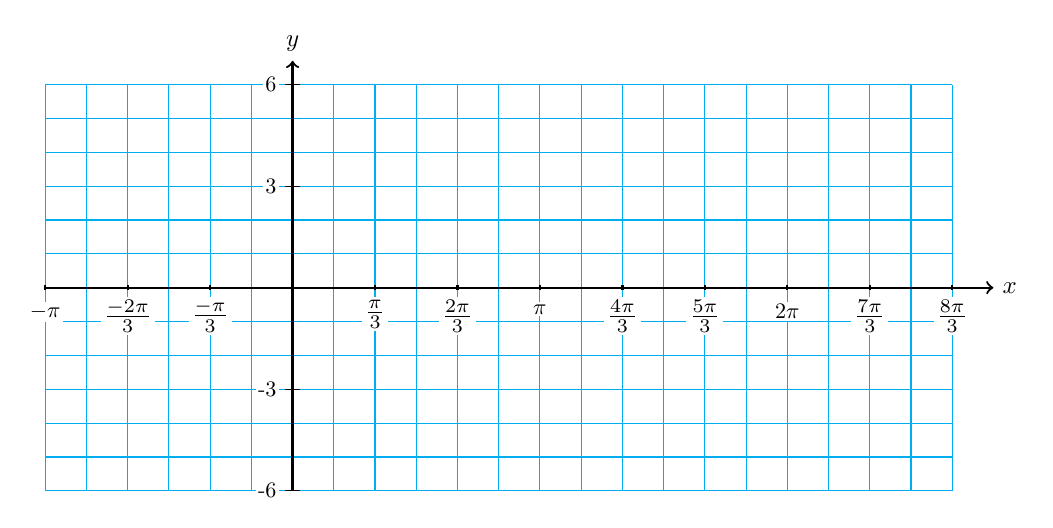
\begin{tikzpicture} [yscale=.43]
\draw[cyan] (-pi,-6) grid[xstep=pi/6, ystep=1] (8*pi/3,6);
\draw[black,thick,->] (-pi,0)--(8.9,0) node[right, scale=.9]{$x$};
\draw[black,thick,->] (0,-6)--(0,6.7) node[above, scale=.9]{$y$};
\foreach \y in {-6,-3,3,6} \draw(.1,\y)--++(-.2,0) node[left, xshift=-2, fill=white, inner sep=1, scale=.8] {\y};
\draw[black,thick] (-pi,.08)--++(0,-.16) node[below, yshift=-4, fill=white, inner sep=1, scale=.8] {$-\pi$};
\draw[black,thick] (pi,.08)--++(0,-.16) node[below, yshift=-4, fill=white, inner sep=1, scale=.8] {$\pi$};
\draw[black,thick] (-2*pi/3,.08)--++(0,-.16) node[below, yshift=-2, fill=white, inner sep=1] {$\frac{-2\pi}{3}$};
\draw[black,thick] (-pi/3,.08)--++(0,-.16) node[below, yshift=-2, fill=white, inner sep=1] {$\frac{-\pi}{3}$};
\draw[black,thick] (pi/3,.08)--++(0,-.16) node[below, yshift=-2, fill=white, inner sep=1] {$\frac{\pi}{3}$};
\draw[black,thick] (2*pi/3,.08)--++(0,-.16) node[below, yshift=-2, fill=white, inner sep=1] {$\frac{2\pi}{3}$};
\draw[black,thick] (4*pi/3,.08)--++(0,-.16) node[below, yshift=-2, fill=white, inner sep=1] {$\frac{4\pi}{3}$};
\draw[black,thick] (5*pi/3,.08)--++(0,-.16) node[below, yshift=-2, fill=white, inner sep=1] {$\frac{5\pi}{3}$};
\draw[black,thick] (2*pi/3,.08)--++(0,-.16) node[below, yshift=-2, fill=white, inner sep=1] {$\frac{2\pi}{3}$};
\draw[black,thick] (2*pi,.08)--++(0,-.16) node[below, yshift=-4, fill=white, inner sep=1, scale=.8] {$2\pi$};
\draw[black,thick] (7*pi/3,.08)--++(0,-.16) node[below, yshift=-2, fill=white, inner sep=1] {$\frac{7\pi}{3}$};
\draw[black,thick] (8*pi/3,.08)--++(0,-.16) node[below, yshift=-2, fill=white, inner sep=1] {$\frac{8\pi}{3}$};
\end{tikzpicture}
\newline


hp7-2-7 cos(x-pi/4)

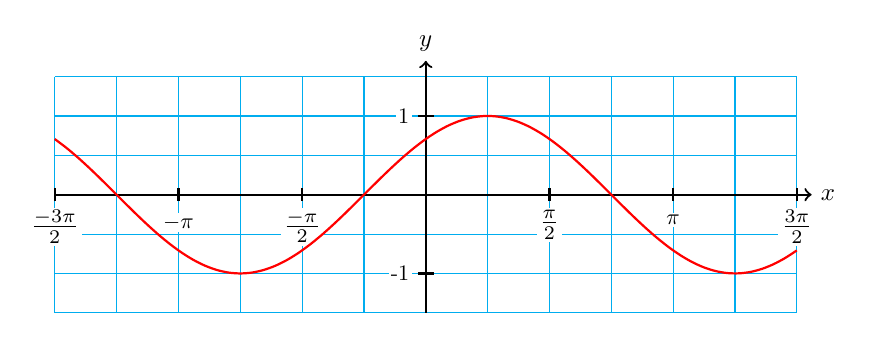
\begin{tikzpicture}
\draw[cyan] (-3*pi/2,-3/2) grid[xstep=pi/4, ystep=1/2] (3*pi/2,3/2);
\draw[black,thick,->] (-3*pi/2,0)--(4.9,0) node[right, scale=.9] {$x$};
\draw[black,thick,->] (0,-3/2)--(0,1.7) node[above, scale=.9] {$y$};
\foreach \y in {-1,1} \draw[black,thick] (.1,\y)--++(-.2,0) node[left, xshift=-2, fill=white, inner sep=1, scale=.8] {\y};
\draw[black,thick] (-3*pi/2,.08)--++(0,-.16) node[below, yshift=-2, fill=white, inner sep=1] {$\frac{-3\pi}{2}$};
\draw[black,thick] (-pi/2,.08)--++(0,-.16) node[below, yshift=-2, fill=white, inner sep=1] {$\frac{-\pi}{2}$};
\draw[black,thick] (pi/2,.08)--++(0,-.16) node[below, yshift=-2, fill=white, inner sep=1] {$\frac{\pi}{2}$};
\draw[black,thick] (3*pi/2,.08)--++(0,-.16) node[below, yshift=-2, fill=white, inner sep=1] {$\frac{3\pi}{2}$};
\draw[black,thick] (-pi,.08)--++(0,-.16) node[below, yshift=-4, fill=white, inner sep=1, scale=.8] {$-\pi$};
\draw[black,thick] (pi,.08)--++(0,-.16) node[below, yshift=-4, fill=white, inner sep=1, scale=.8] {$\pi$};
\draw[samples=65, domain=-3*pi/2:3*pi/2, variable=\x,smooth, red, thick] plot (\x,{cos(deg(\x-pi/4))});
\end{tikzpicture}
\newline


hp7-2-8 cos(x-pi/3)

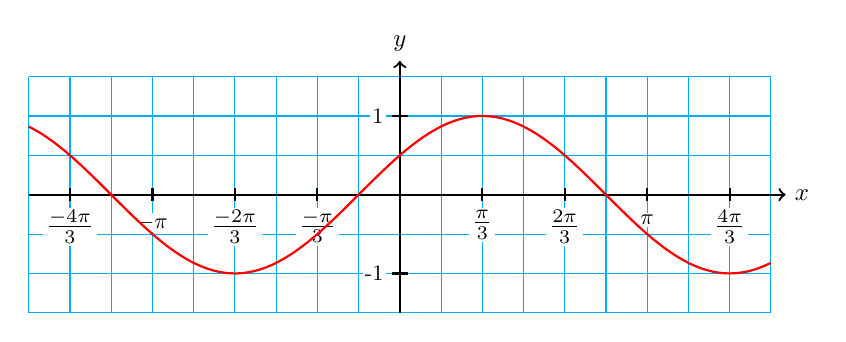
\begin{tikzpicture}
\draw[cyan] (-3*pi/2,-3/2) grid[xstep=pi/6, ystep=1/2] (3*pi/2,3/2);
\draw[black,thick,->] (-3*pi/2,0)--(4.9,0) node[right, scale=.9] {$x$};
\draw[black,thick,->] (0,-3/2)--(0,1.7) node[above, scale=.9] {$y$};
\foreach \y in {-1,1} \draw[black,thick] (.1,\y)--++(-.2,0) node[left, xshift=-2, fill=white, inner sep=1, scale=.8] {\y};
\draw[black,thick] (-4*pi/3,.08)--++(0,-.16) node[below, yshift=-2, fill=white, inner sep=1] {$\frac{-4\pi}{3}$};
\draw[black,thick] (-2*pi/3,.08)--++(0,-.16) node[below, yshift=-2, fill=white, inner sep=1] {$\frac{-2\pi}{3}$};
\draw[black,thick] (-pi/3,.08)--++(0,-.16) node[below, yshift=-2, fill=white, inner sep=1] {$\frac{-\pi}{3}$};
\draw[black,thick] (pi/3,.08)--++(0,-.16) node[below, yshift=-2, fill=white, inner sep=1] {$\frac{\pi}{3}$};
\draw[black,thick] (2*pi/3,.08)--++(0,-.16) node[below, yshift=-2, fill=white, inner sep=1] {$\frac{2\pi}{3}$};
\draw[black,thick] (4*pi/3,.08)--++(0,-.16) node[below, yshift=-2, fill=white, inner sep=1] {$\frac{4\pi}{3}$};
\draw[black,thick] (-pi,.08)--++(0,-.16) node[below, yshift=-4, fill=white, inner sep=1, scale=.8] {$-\pi$};
\draw[black,thick] (pi,.08)--++(0,-.16) node[below, yshift=-4, fill=white, inner sep=1, scale=.8] {$\pi$};
\draw[samples=65, domain=-3*pi/2:3*pi/2, variable=\x,smooth, red, thick] plot (\x,{cos(deg(\x-pi/3))});
\end{tikzpicture}
\newline


hp7-2-9 tan(x-pi/3)

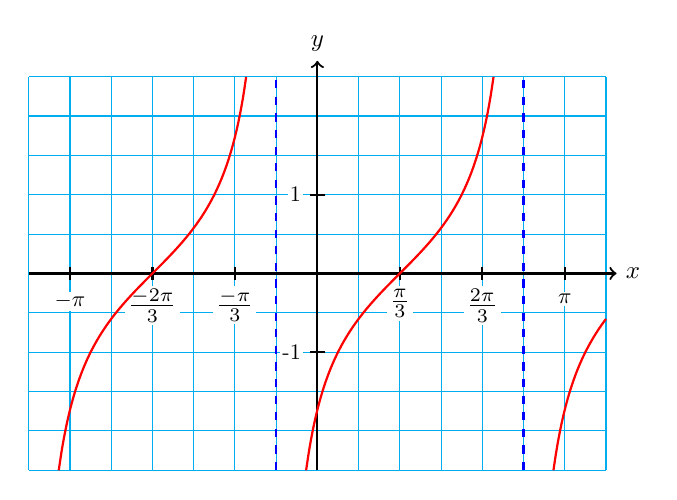
\begin{tikzpicture}
\draw[cyan] (-7*pi/6,-5/2) grid[xstep=pi/6, ystep=1/2] (7*pi/6,5/2);
\draw[black,thick,->] (-7*pi/6,0)--(3.8,0) node[right, scale=.9] {$x$};
\draw[black,thick,->] (0,-5/2)--(0,2.7) node[above, scale=.9] {$y$};
\foreach \y in {-1,1} \draw[black,thick] (.1,\y)--++(-.2,0) node[left, xshift=-2, fill=white, inner sep=1, scale=.8] {\y};
\draw[black,thick] (-2*pi/3,.08)--++(0,-.16) node[below, yshift=-2, fill=white, inner sep=1] {$\frac{-2\pi}{3}$};
\draw[black,thick] (-pi/3,.08)--++(0,-.16) node[below, yshift=-2, fill=white, inner sep=1] {$\frac{-\pi}{3}$};
\draw[black,thick] (pi/3,.08)--++(0,-.16) node[below, yshift=-2, fill=white, inner sep=1] {$\frac{\pi}{3}$};
\draw[black,thick] (2*pi/3,.08)--++(0,-.16) node[below, yshift=-2, fill=white, inner sep=1] {$\frac{2\pi}{3}$};
\draw[black,thick] (-pi,.08)--++(0,-.16) node[below, yshift=-4, fill=white, inner sep=1, scale=.8] {$-\pi$};
\draw[black,thick] (pi,.08)--++(0,-.16) node[below, yshift=-4, fill=white, inner sep=1, scale=.8] {$\pi$};
\draw[blue,thick,dashed] (-pi/6,-5/2)--++(0,5);
\draw[blue,thick,dashed] (5*pi/6,-5/2)--++(0,5);
\draw[samples=65, domain={-atan(5/2)*pi/180}:{atan(5/2)*pi/180}, variable=\x,smooth, red, thick] plot (\x+pi/3,{tan(deg(\x))});
\draw[samples=65, domain={-atan(5/2)*pi/180}:{atan(5/2)*pi/180}, variable=\x,smooth, red, thick] plot (\x-2*pi/3,{tan(deg(\x))});
\draw[samples=65, domain={-atan(5/2)*pi/180+4*pi/3}:7*pi/6, variable=\x,smooth, red, thick] plot (\x,{tan(deg(\x-pi/3))});
\end{tikzpicture}
\newline


hp7-2-10 tan(x+pi/6)

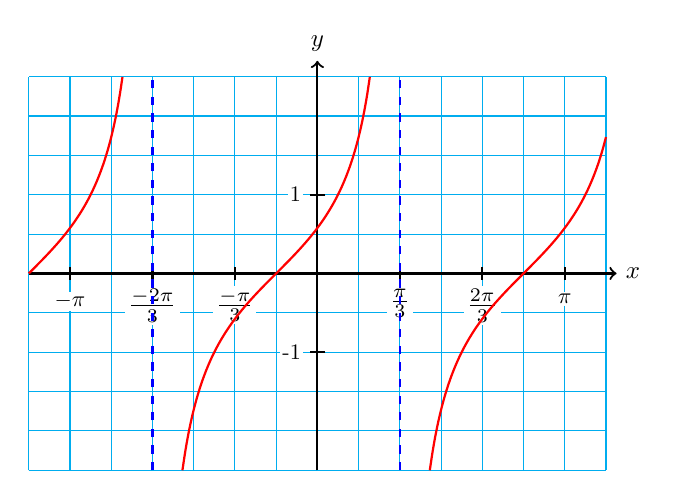
\begin{tikzpicture}
\draw[cyan] (-7*pi/6,-5/2) grid[xstep=pi/6, ystep=1/2] (7*pi/6,5/2);
\draw[black,thick,->] (-7*pi/6,0)--(3.8,0) node[right, scale=.9] {$x$};
\draw[black,thick,->] (0,-5/2)--(0,2.7) node[above, scale=.9] {$y$};
\foreach \y in {-1,1} \draw[black,thick] (.1,\y)--++(-.2,0) node[left, xshift=-2, fill=white, inner sep=1, scale=.8] {\y};
\draw[black,thick] (-2*pi/3,.08)--++(0,-.16) node[below, yshift=-2, fill=white, inner sep=1] {$\frac{-2\pi}{3}$};
\draw[black,thick] (-pi/3,.08)--++(0,-.16) node[below, yshift=-2, fill=white, inner sep=1] {$\frac{-\pi}{3}$};
\draw[black,thick] (pi/3,.08)--++(0,-.16) node[below, yshift=-2, fill=white, inner sep=1] {$\frac{\pi}{3}$};
\draw[black,thick] (2*pi/3,.08)--++(0,-.16) node[below, yshift=-2, fill=white, inner sep=1] {$\frac{2\pi}{3}$};
\draw[black,thick] (-pi,.08)--++(0,-.16) node[below, yshift=-4, fill=white, inner sep=1, scale=.8] {$-\pi$};
\draw[black,thick] (pi,.08)--++(0,-.16) node[below, yshift=-4, fill=white, inner sep=1, scale=.8] {$\pi$};
\draw[blue,thick,dashed] (-2*pi/3,-5/2)--++(0,5);
\draw[blue,thick,dashed] (pi/3,-5/2)--++(0,5);
\draw[samples=65, domain={-atan(5/2)*pi/180}:{atan(5/2)*pi/180}, variable=\x,smooth, red, thick] plot (\x-pi/6,{tan(deg(\x))});
\draw[samples=65, domain={-atan(5/2)*pi/180+5*pi/6}:7*pi/6, variable=\x,smooth, red, thick] plot (\x,{tan(deg(\x+pi/6))});
\draw[samples=65, domain={-7*pi/6}:{atan(5/2)*pi/180-7*pi/6}, variable=\x,smooth, red, thick] plot (\x,{tan(deg(\x+pi/6))});
\end{tikzpicture}
\newline


hp7-2-11 grid

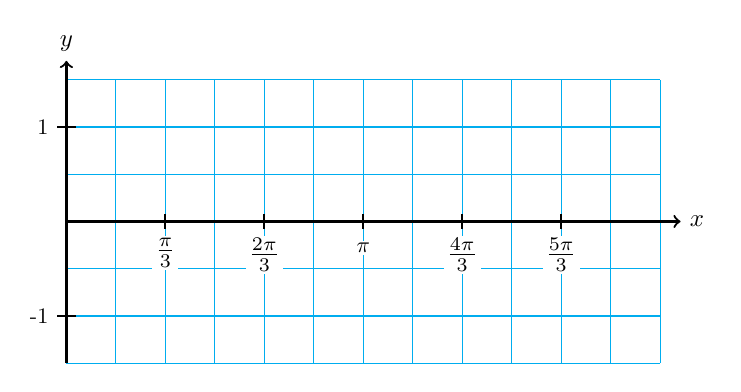
\begin{tikzpicture} [scale=1.2]
\draw[cyan] (0,-3/2) grid[xstep=pi/6, ystep=1/2] (2*pi,3/2);
\draw[black,thick,->] (0,0)--(6.5,0) node[right, scale=.9] {$x$};
\draw[black,thick,->] (0,-3/2)--(0,1.7) node[above, scale=.9] {$y$};
\foreach \y in {-1,1} \draw[black,thick] (.1,\y)--++(-.2,0) node[left, xshift=-2, fill=white, inner sep=1, scale=.8] {\y};
\draw[black,thick] (pi/3,.08)--++(0,-.16) node[below, yshift=-2, fill=white, inner sep=1] {$\frac{\pi}{3}$};
\draw[black,thick] (2*pi/3,.08)--++(0,-.16) node[below, yshift=-2, fill=white, inner sep=1] {$\frac{2\pi}{3}$};
\draw[black,thick] (4*pi/3,.08)--++(0,-.16) node[below, yshift=-2, fill=white, inner sep=1] {$\frac{4\pi}{3}$};
\draw[black,thick] (5*pi/3,.08)--++(0,-.16) node[below, yshift=-2, fill=white, inner sep=1] {$\frac{5\pi}{3}$};
\draw[black,thick] (pi,.08)--++(0,-.16) node[below, yshift=-4, fill=white, inner sep=1, scale=.8] {$\pi$};
\end{tikzpicture}
\newline


hp7-2-11ans cos(2x-pi/3)

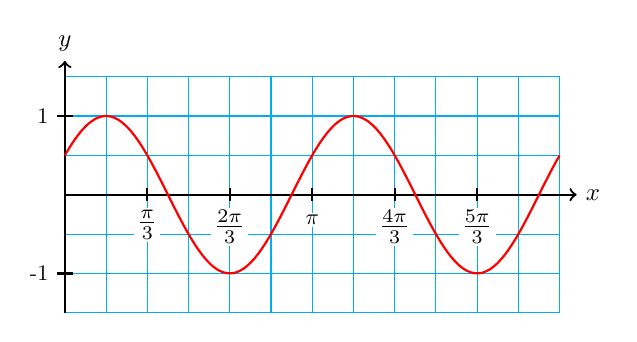
\begin{tikzpicture}
\draw[cyan] (0,-3/2) grid[xstep=pi/6, ystep=1/2] (2*pi,3/2);
\draw[black,thick,->] (0,0)--(6.5,0) node[right, scale=.9] {$x$};
\draw[black,thick,->] (0,-3/2)--(0,1.7) node[above, scale=.9] {$y$};
\foreach \y in {-1,1} \draw[black,thick] (.1,\y)--++(-.2,0) node[left, xshift=-2, fill=white, inner sep=1, scale=.8] {\y};
\draw[black,thick] (pi/3,.08)--++(0,-.16) node[below, yshift=-2, fill=white, inner sep=1] {$\frac{\pi}{3}$};
\draw[black,thick] (2*pi/3,.08)--++(0,-.16) node[below, yshift=-2, fill=white, inner sep=1] {$\frac{2\pi}{3}$};
\draw[black,thick] (4*pi/3,.08)--++(0,-.16) node[below, yshift=-2, fill=white, inner sep=1] {$\frac{4\pi}{3}$};
\draw[black,thick] (5*pi/3,.08)--++(0,-.16) node[below, yshift=-2, fill=white, inner sep=1] {$\frac{5\pi}{3}$};
\draw[black,thick] (pi,.08)--++(0,-.16) node[below, yshift=-4, fill=white, inner sep=1, scale=.8] {$\pi$};
\draw[samples=65, domain=0:2*pi, variable=\x,smooth, red, thick] plot (\x,{cos(deg(2*\x-pi/3))});
\end{tikzpicture}
\newline


hp7-2-13 grid

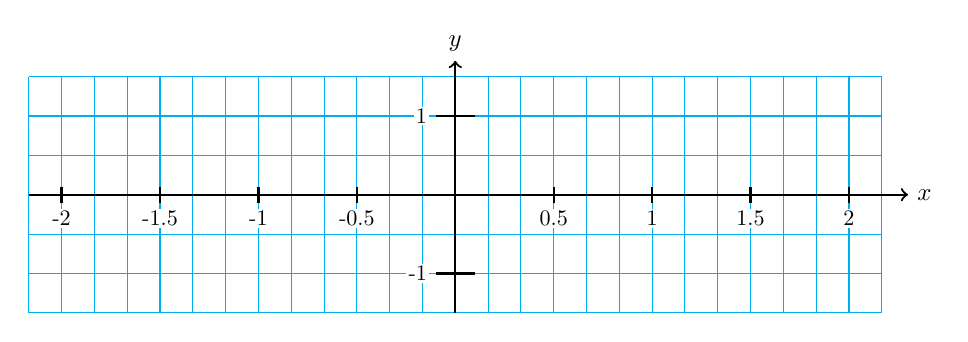
\begin{tikzpicture} [xscale=2.5]
\draw[cyan] (-13/6,-3/2) grid[xstep=1/6, ystep=1/2] (13/6,3/2);
\draw[black,thick,->] (-13/6,0)--(2.3,0) node[right, scale=.9] {$x$};
\draw[black,thick,->] (0,-3/2)--(0,1.7) node[above, scale=.9] {$y$};
\foreach \x in {-2, -1.5,-1,-0.5,0.5,1,1.5,2} \draw[black,thick] (\x,.1)--++(0,-.2) node[below, yshift=-2, fill=white, inner sep=1, scale=.8] {\x};
\foreach \y in {-1,1} \draw[black,thick] (.1,\y)--++(-.2,0) node[left, xshift=-2, fill=white, inner sep=1, scale=.8] {\y};
\end{tikzpicture}
\newline


hp7-2-13ans grid sin(pi x + pi/3)

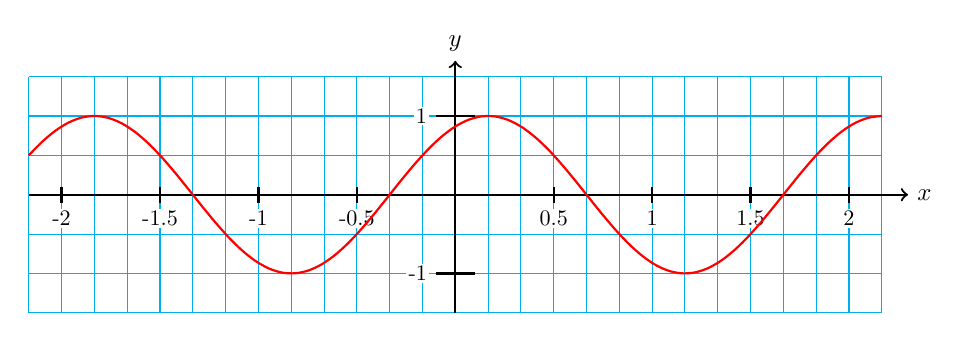
\begin{tikzpicture} [xscale=2.5]
\draw[cyan] (-13/6,-3/2) grid[xstep=1/6, ystep=1/2] (13/6,3/2);
\draw[black,thick,->] (-13/6,0)--(2.3,0) node[right, scale=.9] {$x$};
\draw[black,thick,->] (0,-3/2)--(0,1.7) node[above, scale=.9] {$y$};
\foreach \x in {-2, -1.5,-1,-0.5,0.5,1,1.5,2} \draw[black,thick] (\x,.1)--++(0,-.2) node[below, yshift=-2, fill=white, inner sep=1, scale=.8] {\x};
\foreach \y in {-1,1} \draw[black,thick] (.1,\y)--++(-.2,0) node[left, xshift=-2, fill=white, inner sep=1, scale=.8] {\y};
\draw[samples=65, domain=-13/6:13/6, variable=\x,smooth, red, thick] plot (\x,{sin(deg(pi*\x+pi/3))});
\end{tikzpicture}
\newline


hp7-2-15 grid

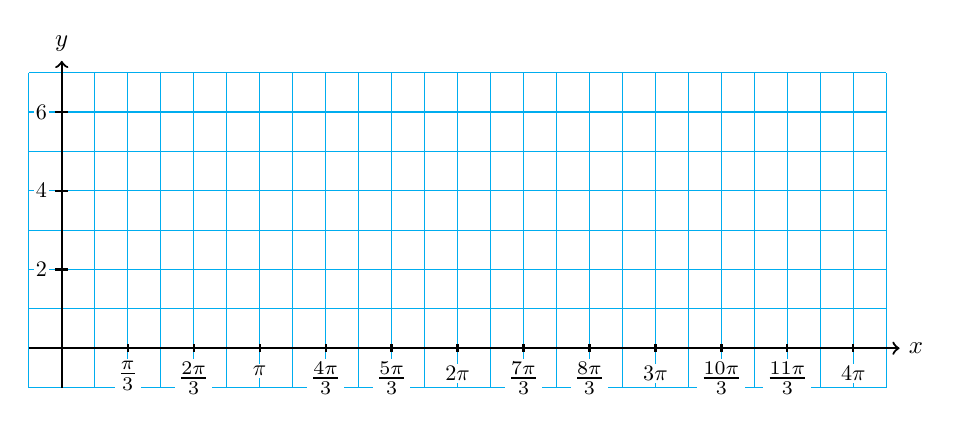
\begin{tikzpicture} [xscale=.8, yscale=.5]
\draw[cyan] (-pi/6,-1) grid[xstep=pi/6, ystep=1] (25*pi/6,7);
\draw[black,thick,->] (-pi/6,0)--(13.3,0) node[right, scale=.9] {$x$};
\draw[black,thick,->] (0,-1)--(0,7.3) node[above, scale=.9] {$y$};

\foreach \y in {2,4,6} \draw[black,thick] (.1,\y)--++(-.2,0) node[left, xshift=-2, fill=white, inner sep=1, scale=.8] {\y};
\draw[black,thick] (pi/3,.1)--++(0,-.2) node[below,yshift=-2, fill=white, inner sep=1] {$\frac{\pi}{3}$};
\draw[black,thick] (2*pi/3,.1)--++(0,-.2) node[below,yshift=-2, fill=white, inner sep=1] {$\frac{2\pi}{3}$};
\draw[black,thick] (4*pi/3,.1)--++(0,-.2) node[below,yshift=-2, fill=white, inner sep=1] {$\frac{4\pi}{3}$};
\draw[black,thick] (5*pi/3,.1)--++(0,-.2) node[below,yshift=-2, fill=white, inner sep=1] {$\frac{5\pi}{3}$};
\draw[black,thick] (7*pi/3,.1)--++(0,-.2) node[below,yshift=-2, fill=white, inner sep=1] {$\frac{7\pi}{3}$};
\draw[black,thick] (8*pi/3,.1)--++(0,-.2) node[below,yshift=-2, fill=white, inner sep=1] {$\frac{8\pi}{3}$};
\draw[black,thick] (10*pi/3,.1)--++(0,-.2) node[below,yshift=-2, fill=white, inner sep=1] {$\frac{10\pi}{3}$};
\draw[black,thick] (11*pi/3,.1)--++(0,-.2) node[below,yshift=-2, fill=white, inner sep=1] {$\frac{11\pi}{3}$};
\draw[black,thick] (pi,.1)--++(0,-.2) node[below,yshift=-4, fill=white, inner sep=1, scale=.8] {$\pi$};
\draw[black,thick] (2*pi,.1)--++(0,-.2) node[below,yshift=-4, fill=white, inner sep=1, scale=.8] {$2\pi$};
\draw[black,thick] (3*pi,.1)--++(0,-.2) node[below,yshift=-4, fill=white, inner sep=1, scale=.8] {$3\pi$};
\draw[black,thick] (4*pi,.1)--++(0,-.2) node[below,yshift=-4, fill=white, inner sep=1, scale=.8] {$4\pi$};
\end{tikzpicture}
\newline


hp7-2-15ans 3sin(x/2 - pi/6) + 4

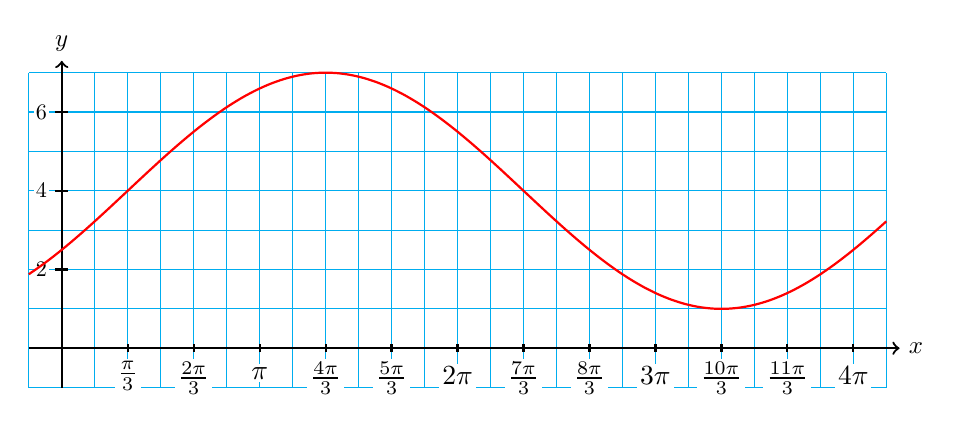
\begin{tikzpicture} [xscale=.8, yscale=.5]
\draw[cyan] (-pi/6,-1) grid[xstep=pi/6, ystep=1] (25*pi/6,7);
\draw[black,thick,->] (-pi/6,0)--(13.3,0) node[right, scale=.9] {$x$};
\draw[black,thick,->] (0,-1)--(0,7.3) node[above, scale=.9] {$y$};
\foreach \y in {2,4,6} \draw[black,thick] (.1,\y)--++(-.2,0) node[left, xshift=-2, fill=white, inner sep=1, scale=.8] {\y};
\draw[black,thick] (pi/3,.1)--++(0,-.2) node[below,yshift=-2, fill=white, inner sep=1] {$\frac{\pi}{3}$};
\draw[black,thick] (2*pi/3,.1)--++(0,-.2) node[below,yshift=-2, fill=white, inner sep=1] {$\frac{2\pi}{3}$};
\draw[black,thick] (4*pi/3,.1)--++(0,-.2) node[below,yshift=-2, fill=white, inner sep=1] {$\frac{4\pi}{3}$};
\draw[black,thick] (5*pi/3,.1)--++(0,-.2) node[below,yshift=-2, fill=white, inner sep=1] {$\frac{5\pi}{3}$};
\draw[black,thick] (7*pi/3,.1)--++(0,-.2) node[below,yshift=-2, fill=white, inner sep=1] {$\frac{7\pi}{3}$};
\draw[black,thick] (8*pi/3,.1)--++(0,-.2) node[below,yshift=-2, fill=white, inner sep=1] {$\frac{8\pi}{3}$};
\draw[black,thick] (10*pi/3,.1)--++(0,-.2) node[below,yshift=-2, fill=white, inner sep=1] {$\frac{10\pi}{3}$};
\draw[black,thick] (11*pi/3,.1)--++(0,-.2) node[below,yshift=-2, fill=white, inner sep=1] {$\frac{11\pi}{3}$};
\draw[black,thick] (pi,.1)--++(0,-.2) node[below,yshift=-4, fill=white, inner sep=1] {$\pi$};
\draw[black,thick] (2*pi,.1)--++(0,-.2) node[below,yshift=-4, fill=white, inner sep=1] {$2\pi$};
\draw[black,thick] (3*pi,.1)--++(0,-.2) node[below,yshift=-4, fill=white, inner sep=1] {$3\pi$};
\draw[black,thick] (4*pi,.1)--++(0,-.2) node[below,yshift=-4, fill=white, inner sep=1] {$4\pi$};
\draw[samples=65, domain=-pi/6:25*pi/6, variable=\x,smooth, red, thick] plot (\x,{3*sin(deg(\x/2 - pi/6))+4});
\end{tikzpicture}
\newline


hp7-2-16 grid

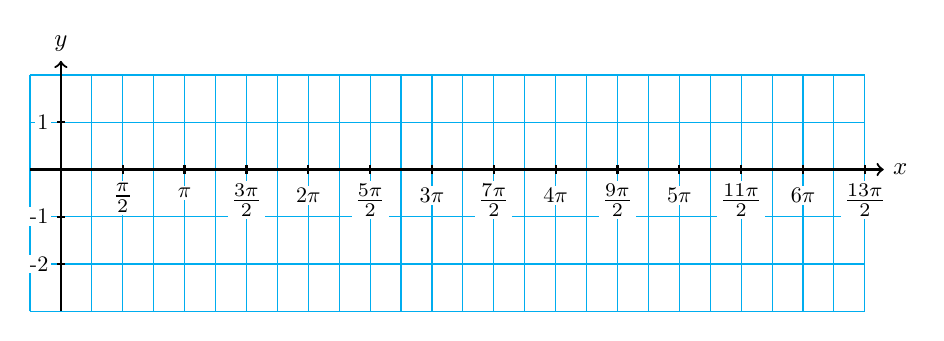
\begin{tikzpicture} [xscale=.5, yscale=.6]
\draw[cyan] (-pi/4,-3) grid[xstep=pi/4, ystep=1] (13*pi/2,2);
\draw[black,thick,->] (-pi/4,0)--(20.9,0) node[right, scale=.9] {$x$};
\draw[black,thick,->] (0,-3)--(0,2.3) node[above, scale=.9] {$y$};

\foreach \y in {-2,-1,1} \draw[black,thick] (.1,\y)--++(-.2,0) node[left, xshift=-2, fill=white, inner sep=1, scale=.8] {\y};
\draw[black,thick] (pi/2,.1)--++(0,-.2) node[below,yshift=-2, fill=white, inner sep=1] {$\frac{\pi}{2}$};
\draw[black,thick] (3*pi/2,.1)--++(0,-.2) node[below,yshift=-2, fill=white, inner sep=1] {$\frac{3\pi}{2}$};
\draw[black,thick] (5*pi/2,.1)--++(0,-.2) node[below,yshift=-2, fill=white, inner sep=1] {$\frac{5\pi}{2}$};
\draw[black,thick] (7*pi/2,.1)--++(0,-.2) node[below,yshift=-2, fill=white, inner sep=1] {$\frac{7\pi}{2}$};
\draw[black,thick] (9*pi/2,.1)--++(0,-.2) node[below,yshift=-2, fill=white, inner sep=1] {$\frac{9\pi}{2}$};
\draw[black,thick] (11*pi/2,.1)--++(0,-.2) node[below,yshift=-2, fill=white, inner sep=1] {$\frac{11\pi}{2}$};
\draw[black,thick] (13*pi/2,.1)--++(0,-.2) node[below,yshift=-2, fill=white, inner sep=1] {$\frac{13\pi}{2}$};
\draw[black,thick] (pi,.1)--++(0,-.2) node[below,yshift=-4, fill=white, inner sep=1, scale=.8] {$\pi$};
\draw[black,thick] (2*pi,.1)--++(0,-.2) node[below,yshift=-4, fill=white, inner sep=1, scale=.8] {$2\pi$};
\draw[black,thick] (3*pi,.1)--++(0,-.2) node[below,yshift=-4, fill=white, inner sep=1, scale=.8] {$3\pi$};
\draw[black,thick] (4*pi,.1)--++(0,-.2) node[below,yshift=-4, fill=white, inner sep=1, scale=.8] {$4\pi$};
\draw[black,thick] (5*pi,.1)--++(0,-.2) node[below,yshift=-4, fill=white, inner sep=1, scale=.8] {$5\pi$};
\draw[black,thick] (6*pi,.1)--++(0,-.2) node[below,yshift=-4, fill=white, inner sep=1, scale=.8] {$6\pi$};
\end{tikzpicture}
\newline


hp7-2-17ans 2 sin(2pi/ (x + 4) )+5

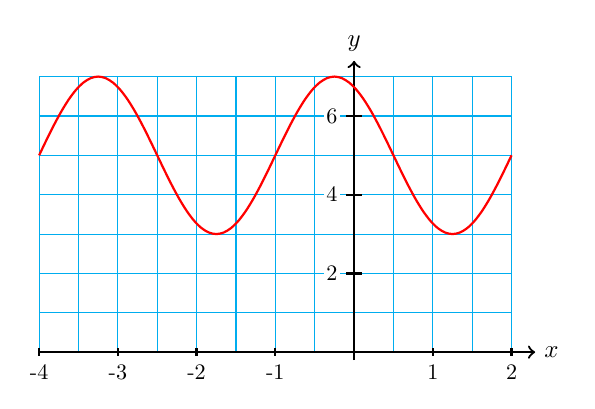
\begin{tikzpicture} [yscale=.5]
\draw[cyan] (-4,0) grid[xstep=1/2, ystep=1] (2,7);
\draw[black,thick,->] (-4,0)--(2.3,0) node[right, scale=.9] {$x$};
\draw[black,thick,->] (0,-.2)--(0,7.4) node[above, scale=.9] {$y$};
\foreach \x in {-4,-2,2,-3,-1,1} \draw[black,thick] (\x,.1)--++(0,-.2) node[below, yshift=-2, fill=white, inner sep=1, scale=.8] {\x};
\foreach \y in {2,4,6} \draw[black,thick] (.1,\y)--++(-.2,0) node[left, xshift=-2, fill=white, inner sep=1, scale=.8] {\y};
\draw[samples=65, domain=-4:2, variable=\x,smooth, red, thick] plot (\x,{2*sin(deg(2*pi/3*(\x+4)))+5});
\end{tikzpicture}
\newline


hp7-2-19ans $y=-5\cos(\frac{\pi x}{180})+12$

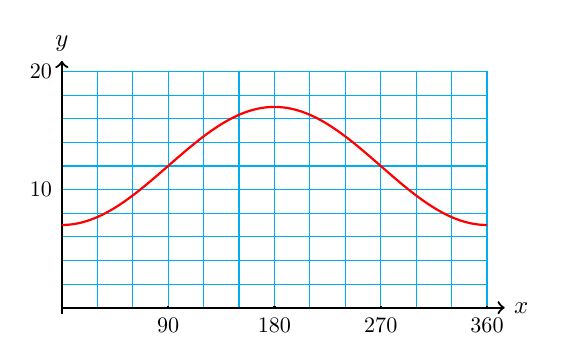
\begin{tikzpicture} [xscale=.015, yscale=.15]
\draw[cyan] (0,0) grid[xstep=30, ystep=2] (360,20);
\draw[black,thick,->] (0,0)--(375,0) node[right, scale=.9] {$x$};
\draw[black,thick,->] (0,-.5)--(0,20.9) node[above, scale=.9] {$y$};
\foreach \x in {90,180,270,360} \draw[black,thick] (\x,.15)--++(0,-.3) node[below, yshift=-2, fill=white, inner sep=1, scale=.8] {\x};
\foreach \y in {10,20} \draw[black,thick] (1,\y)--++(-2,0) node[left, xshift=-2, fill=white, inner sep=1, scale=.8] {\y};
\draw[samples=65, domain=0:360, variable=\x,smooth, red, thick] plot (\x,{-5*cos(\x)+12});
\end{tikzpicture}
\newline


hp7-2-21 3cos(x + pi/6)

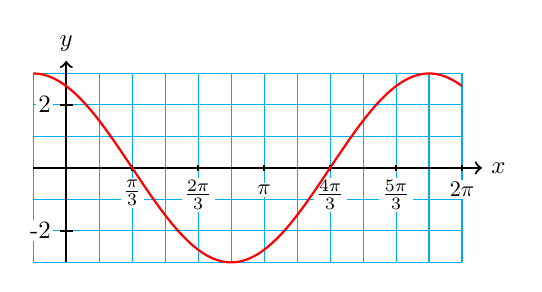
\begin{tikzpicture} [xscale=.8,yscale=.4]
\draw[cyan] (-pi/6,-3) grid[xstep=pi/6] (2*pi,3);
\draw[black,thick,->] (-pi/6,0)--(6.6,0) node[right, scale=.9] {$x$};
\draw[black,thick,->] (0,-3)--(0,3.4) node[above, scale=.9] {$y$};
\foreach \y in {-2,2} \draw[black,thick] (.1,\y)--++(-.2,0) node[left, xshift=-2, fill=white, inner sep=1, scale=.9] {\y};
\draw[black,thick] (pi/3,.1)--++(0,-.2) node[below, yshift=-2, fill=white, inner sep=1, scale=.9] {$\frac{\pi}{3}$};
\draw[black,thick] (2*pi/3,.1)--++(0,-.2) node[below, yshift=-2, fill=white, inner sep=1, scale=.9] {$\frac{2\pi}{3}$};
\draw[black,thick] (pi,.1)--++(0,-.2) node[below, yshift=-4, fill=white, inner sep=1, scale=.8] {$\pi$};
\draw[black,thick] (4*pi/3,.1)--++(0,-.2) node[below, yshift=-2, fill=white, inner sep=1, scale=.9] {$\frac{4\pi}{3}$};
\draw[black,thick] (5*pi/3,.1)--++(0,-.2) node[below, yshift=-2, fill=white, inner sep=1, scale=.9] {$\frac{5\pi}{3}$};
\draw[black,thick] (2*pi,.1)--++(0,-.2) node[below, yshift=-3, fill=white, inner sep=1, scale=.8] {$2\pi$};
\draw[samples=65, domain=-pi/6:2*pi, variable=\x,smooth, red, thick] plot (\x,{3*cos( deg(\x+pi/6) )});
\end{tikzpicture}
\newline


hp7-2-22 4sin(x - pi/4)

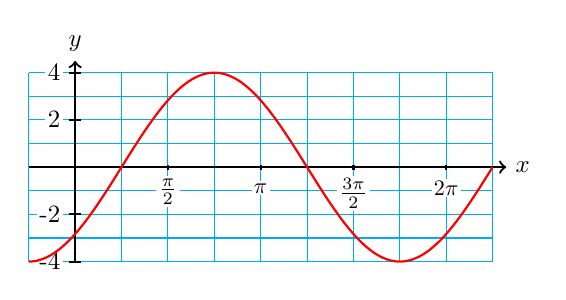
\begin{tikzpicture} [xscale=.75,yscale=.3]
\draw[cyan] (-pi/4,-4) grid[xstep=pi/4] (9*pi/4,4);
\draw[black,thick,->] (-pi/4,0)--(7.3,0) node[right, scale=.9] {$x$};
\draw[black,thick,->] (0,-4)--(0,4.5) node[above, scale=.9] {$y$};
\foreach \y in {-2,2,-4,4} \draw[black,thick] (.1,\y)--++(-.2,0) node[left, xshift=-2, fill=white, inner sep=1, scale=.9] {\y};
\draw[black,thick] (pi/2,.1)--++(0,-.2) node[below, yshift=-2, fill=white, inner sep=1, scale=.9] {$\frac{\pi}{2}$};
\draw[black,thick] (3*pi/2,.1)--++(0,-.2) node[below, yshift=-2, fill=white, inner sep=1, scale=.9] {$\frac{3\pi}{2}$};
\draw[black,thick] (pi,.1)--++(0,-.2) node[below, yshift=-4, fill=white, inner sep=1, scale=.8] {$\pi$};
\draw[black,thick] (2*pi,.1)--++(0,-.2) node[below, yshift=-3, fill=white, inner sep=1, scale=.8] {$2\pi$};
\draw[samples=65, domain=-pi/4:9*pi/4, variable=\x,smooth, red, thick] plot (\x,{4*sin( deg(\x-pi/4) )});
\end{tikzpicture}
\newline


hp7-2-23 -2cos(2x )

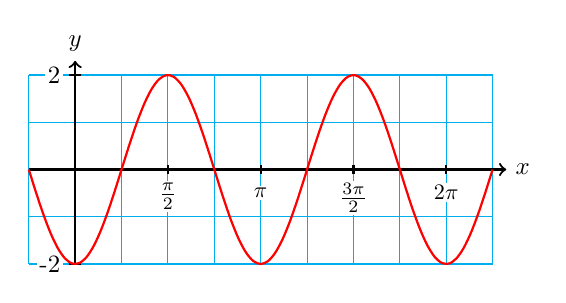
\begin{tikzpicture} [xscale=.75,yscale=.6]
\draw[cyan] (-pi/4,-2) grid[xstep=pi/4] (9*pi/4,2);
\draw[black,thick,->] (-pi/4,0)--(7.3,0) node[right, scale=.9] {$x$};
\draw[black,thick,->] (0,-2)--(0,2.3) node[above, scale=.9] {$y$};
\foreach \y in {-2,2} \draw[black,thick] (.1,\y)--++(-.2,0) node[left, xshift=-2, fill=white, inner sep=1, scale=.9] {\y};
\draw[black,thick] (pi/2,.1)--++(0,-.2) node[below, yshift=-2, fill=white, inner sep=1, scale=.9] {$\frac{\pi}{2}$};
\draw[black,thick] (3*pi/2,.1)--++(0,-.2) node[below, yshift=-2, fill=white, inner sep=1, scale=.9] {$\frac{3\pi}{2}$};
\draw[black,thick] (pi,.1)--++(0,-.2) node[below, yshift=-4, fill=white, inner sep=1, scale=.8] {$\pi$};
\draw[black,thick] (2*pi,.1)--++(0,-.2) node[below, yshift=-3, fill=white, inner sep=1, scale=.8] {$2\pi$};
\draw[samples=65, domain=-pi/4:9*pi/4, variable=\x,smooth, red, thick] plot (\x,{-2*cos( deg(2*\x) )});
\end{tikzpicture}
\newline


hp7-2-24 -3cos(3x 6)

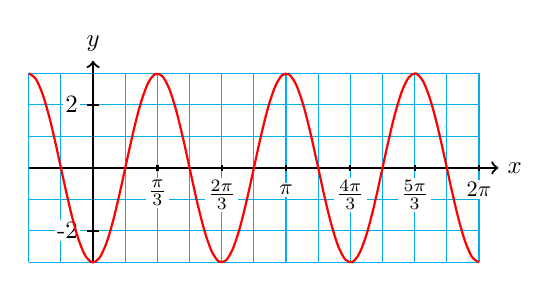
\begin{tikzpicture} [xscale=.78,yscale=.4]
\draw[cyan] (-pi/3,-3) grid[xstep=pi/6] (2*pi,3);
\draw[black,thick,->] (-pi/3,0)--(6.6,0) node[right, scale=.9] {$x$};
\draw[black,thick,->] (0,-3)--(0,3.4) node[above, scale=.9] {$y$};
\foreach \y in {-2,2} \draw[black,thick] (.1,\y)--++(-.2,0) node[left, xshift=-2, fill=white, inner sep=1, scale=.9] {\y};
\draw[black,thick] (pi/3,.1)--++(0,-.2) node[below, yshift=-2, fill=white, inner sep=1, scale=.9] {$\frac{\pi}{3}$};
\draw[black,thick] (2*pi/3,.1)--++(0,-.2) node[below, yshift=-2, fill=white, inner sep=1, scale=.9] {$\frac{2\pi}{3}$};
\draw[black,thick] (pi,.1)--++(0,-.2) node[below, yshift=-4, fill=white, inner sep=1, scale=.8] {$\pi$};
\draw[black,thick] (4*pi/3,.1)--++(0,-.2) node[below, yshift=-2, fill=white, inner sep=1, scale=.9] {$\frac{4\pi}{3}$};
\draw[black,thick] (5*pi/3,.1)--++(0,-.2) node[below, yshift=-2, fill=white, inner sep=1, scale=.9] {$\frac{5\pi}{3}$};
\draw[black,thick] (2*pi,.1)--++(0,-.2) node[below, yshift=-3, fill=white, inner sep=1, scale=.8] {$2\pi$};
\draw[samples=65, domain=-pi/3:2*pi, variable=\x,smooth, red, thick] plot (\x,{-3*cos( deg(3*\x) )});
\end{tikzpicture}
\newline


hp7-2-25 -4cos( 1/4 (x - pi/3))

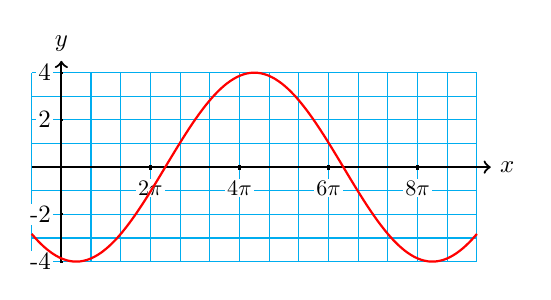
\begin{tikzpicture} [xscale=.18,yscale=.3]
\draw[cyan] (-2*pi/3,-4) grid[xstep=2*pi/3] (28*pi/3,4);
\draw[black,thick,->] (-2*pi/3,0)--(30.3,0) node[right, scale=.9] {$x$};
\draw[black,thick,->] (0,-4)--(0,4.5) node[above, scale=.9] {$y$};
\foreach \y in {-2,2,-4,4} \draw[black,thick] (.1,\y)--++(-.2,0) node[left, xshift=-2, fill=white, inner sep=1, scale=.9] {\y};
\foreach \x [evaluate=\x as \xi using (pi*\x)] in {2,4,6,8} \draw[black,thick] (\xi,.1)--++(0,-.2) node[below, yshift=-3, fill=white, inner sep=1, scale=.8] {$\x\pi$};
\draw[samples=65, domain=-2*pi/3:28*pi/3, variable=\x,smooth, red, thick] plot (\x,{-4*cos( deg(\x/4 -pi/12) )});
\end{tikzpicture}
\newline


hp7-2-26 -2sin(.5(x+pi/6) )

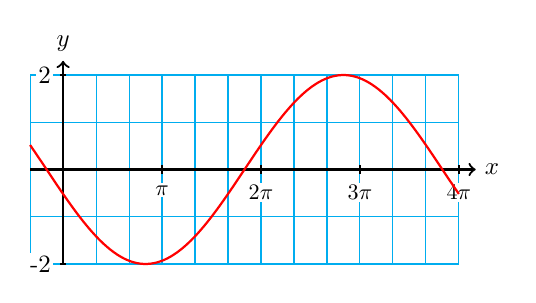
\begin{tikzpicture} [xscale=.4,yscale=.6]
\draw[cyan] (-pi/3,-2) grid[xstep=pi/3] (4*pi,2);
\draw[black,thick,->] (-pi/3,0)--(13.1,0) node[right, scale=.9] {$x$};
\draw[black,thick,->] (0,-2)--(0,2.3) node[above, scale=.9] {$y$};
\foreach \y in {-2,2} \draw[black,thick] (.1,\y)--++(-.2,0) node[left, xshift=-2, fill=white, inner sep=1, scale=.9] {\y};
\draw[black,thick] (pi,.1)--++(0,-.2) node[below, yshift=-3, fill=white, inner sep=1, scale=.8] {$\pi$};
\foreach \x [evaluate=\x as \xi using (pi*\x)] in {2,3,4} \draw[black,thick] (\xi,.1)--++(0,-.2) node[below, yshift=-3, fill=white, inner sep=1, scale=.8] {$\x\pi$};
\draw[samples=65, domain=-pi/3:4*pi, variable=\x,smooth, red, thick] plot (\x,{-2*sin( deg(1/2*(\x+pi/6)) )});
\end{tikzpicture}
\newline


hp7-2-27ans $-36.95 \cos (\frac{\pi}{6} m)+35.35$

\begin{tikzpicture} [xscale=.2, yscale=.03]
\draw[cyan] (0,0) grid[xstep=2, ystep=10] (24,70);
\draw[black,thick,->,>=stealth'] (0,0)--(25.5,0) node[right, scale=.8] {$m$};
\draw[black,thick,->,>=stealth'] (0,-5)--(0,80) node[above, scale=.8] {$T$};
\foreach \x in {4,8,...,24} \draw[black,thick] (\x,3)--++(0,-6) node[below, yshift=-2, scale=.8] {\x};
\foreach \y in {20,40,60} \draw[black,thick] (.2,\y)--++(-.4,0) node[left, scale=.8] {\y};
\draw[samples=65, domain=0:24, variable=\x,smooth, red, thick] plot (\x,{ -36.95 *cos( 30*\x) +35.35 });
\node[scale=.9] at (12,75) {high};
\node[scale=.9, fill=white, inner sep=1] at (12,30) {low};
\draw[blue, ->,>=stealth'] (10,75) --  (6.8,73);
\draw[blue, ->,>=stealth'] (14,75) -- (17,73);
\path (10,28) edge [out=240, in=280,->,>=stealth', blue]  (0.3,-4);
\path (14,28) edge [out=-60, in=-100,->,>=stealth', blue]  (23.7,-4);
\end{tikzpicture}
\newline	


hp7-2-29ans $ h(t)=1.4-1.4\cos(0.51t) $

\begin{tikzpicture} [xscale=.2, yscale=.8]
\draw[cyan] (0,0) grid[xstep=2, ystep=1/2] (24,3);
\draw[black,thick,->,>=stealth'] (0,0)--(26,0) node[right, scale=.8] {$t$};
\draw[black,thick,->,>=stealth'] (0,-.1)--(0,3.3) node[above, scale=.8] {$h$};
\foreach \x in {4,8,...,24} \draw[black,thick] (\x,.1)--++(0,-.2) node[below, yshift=-2, scale=.8] {\x};
\foreach \y in {1,2,3} \draw[black,thick] (.2,\y)--++(-.4,0) node[left, scale=.8] {\y};
\draw[samples=65, domain=0:24.7, variable=\x,smooth, red, thick] plot (\x,{ 1.4-1.4 *cos( deg(0.51*\x) ) });
\node[scale=.9, fill=white, inner sep=1] at (12.32,2.9) {high};
\node[scale=.9, fill=white, inner sep=1] at (12.32,1.5) {low};
\draw[blue, ->,>=stealth'] (10.32,2.9) --  (6.8,2.8);
\draw[blue, ->,>=stealth'] (14,2.9) -- (17,2.8);
\path (10.32,1.4) edge [out=200, in=355,->,>=stealth', blue]  (0.3,-.1);
\path (14,1.4) edge [out=-20, in=-175,->,>=stealth', blue]  (24.3,-.1);
\draw[blue,  ->,>=stealth'] (12.32,1.2) --  ++(0.,-1.1);
\end{tikzpicture}
\newline	






\end{document}
